% Options for packages loaded elsewhere
\PassOptionsToPackage{unicode}{hyperref}
\PassOptionsToPackage{hyphens}{url}
%
\documentclass[10pt, a4page]{report}
\usepackage{amsmath,amssymb}
\usepackage{lmodern}
\usepackage{ifxetex,ifluatex}
\usepackage{float}
\usepackage{caption}
\usepackage{subcaption}
\ifnum 0\ifxetex 1\fi\ifluatex 1\fi=0 % if pdftex
  \usepackage[T1]{fontenc}
  \usepackage[utf8]{inputenc}
  \usepackage{textcomp} % provide euro and other symbols
\else % if luatex or xetex
  \usepackage{unicode-math}
  \defaultfontfeatures{Scale=MatchLowercase}
  \defaultfontfeatures[\rmfamily]{Ligatures=TeX,Scale=1}
\fi
% Use upquote if available, for straight quotes in verbatim environments
\IfFileExists{upquote.sty}{\usepackage{upquote}}{}
\IfFileExists{microtype.sty}{% use microtype if available
  \usepackage[]{microtype}
  \UseMicrotypeSet[protrusion]{basicmath} % disable protrusion for tt fonts
}{}
\makeatletter
\@ifundefined{KOMAClassName}{% if non-KOMA class
  \IfFileExists{parskip.sty}{%
    \usepackage{parskip}
  }{% else
    \setlength{\parindent}{0pt}
    \setlength{\parskip}{6pt plus 2pt minus 1pt}}
}{% if KOMA class
  \KOMAoptions{parskip=half}}
\makeatother
\usepackage{xcolor}
\IfFileExists{xurl.sty}{\usepackage{xurl}}{} % add URL line breaks if available
\IfFileExists{bookmark.sty}{\usepackage{bookmark}}{\usepackage{hyperref}}
\hypersetup{
  hidelinks,
  pdfcreator={LaTeX via pandoc}}
\urlstyle{same} % disable monospaced font for URLs
\usepackage{longtable,booktabs,array}
\usepackage{calc} % for calculating minipage widths
% Correct order of tables after \paragraph or \subparagraph
\usepackage{etoolbox}
\makeatletter
\patchcmd\longtable{\par}{\if@noskipsec\mbox{}\fi\par}{}{}
\makeatother
% Allow footnotes in longtable head/foot
\IfFileExists{footnotehyper.sty}{\usepackage{footnotehyper}}{\usepackage{footnote}}
\makesavenoteenv{longtable}
\usepackage{graphicx}
\makeatletter
\def\maxwidth{\ifdim\Gin@nat@width>\linewidth\linewidth\else\Gin@nat@width\fi}
\def\maxheight{\ifdim\Gin@nat@height>\textheight\textheight\else\Gin@nat@height\fi}
\makeatother
% Scale images if necessary, so that they will not overflow the page
% margins by default, and it is still possible to overwrite the defaults
% using explicit options in \includegraphics[width, height, ...]{}
\setkeys{Gin}{width=\maxwidth,height=\maxheight,keepaspectratio}
% Set default figure placement to htbp
\makeatletter
\def\fps@figure{htbp}
\makeatother
\setlength{\emergencystretch}{3em} % prevent overfull lines
\providecommand{\tightlist}{%
  \setlength{\itemsep}{0pt}\setlength{\parskip}{0pt}}
\setcounter{secnumdepth}{-\maxdimen} % remove section numbering
\ifluatex
  \usepackage{selnolig}  % disable illegal ligatures
\fi

%Custom titling

\usepackage{titling}

% set up \maketitle to accept a new item
\pretitle{\begin{center}\placetitlepicture\Huge}
\posttitle{\par\lineskip 1em\placesubtitle\end{center}\vskip 3em}
\preauthor{\begin{center}
        \large \lineskip 3em%
        \begin{tabular}[t]{c}}
\postauthor{\end{tabular}\par\placeprofessor\end{center}}
\predate{\begin{center}\large\vskip 3em}
\postdate{\par\placeversion\par\end{center}}

% commands for including the picture
\newcommand{\titlepicture}[2][]{%
  \renewcommand\placetitlepicture{%
    \includegraphics[#1]{#2}\par\medskip
  }%
}
\newcommand{\placetitlepicture}{} % initialization

% commands for including the subtitle
\newcommand{\subtitle}[2][]{%
  \renewcommand\placesubtitle{%
    \Large #2\par\medskip
  }%
}
\newcommand{\placesubtitle}{} % initialization

% commands for including the professor
\newcommand{\professor}[2][]{%
  \renewcommand\placeprofessor{%
    \large Professor: #2\par\medskip
  }%
}
\newcommand{\placeprofessor}{} % initialization

% commands for including the version
\newcommand{\version}[2][]{%
  \renewcommand\placeversion{%
    \large Version: #2\par\medskip
  }%
}
\newcommand{\placeversion}{} % initialization
\graphicspath{ {assets/dd/} }

\titlepicture[width=0.75\textwidth]{../polimi_logo}
\title{Design Document}
\subtitle{Customers Line-up}
\author{\href{https://github.com/ferrohd}{Alessandro Ferrara} -
\href{https://github.com/lorenzofratus}{Lorenzo Fratus}}
\professor{Elisabetta di Nitto}
\date{December 24, 2020}
\version{0.2}

\begin{document}

\maketitle

\tableofcontents

\chapter{1. Introduction}

\section{A. Purpose}

The purpose of this document is to provide an overall guidance to the architecture of the software product and therefore it is primarily addressed to the software development team.

More precisely, the document presents an overview of the high level architecture (defining the main components and their interaction) and additional details on the runtime behaviour and the user interface of the application.

Finally, it includes a plan for the implementation, integration and testing activity.

Together with the RASD, this document has the purpose to guide the developers in the realization of the software called Customers Line-up.

\section{B. Scope}

The software wants to foster a safe shopping experience by providing a customer flow control system. This system should allow the users to avoid crowds both inside and outside the stores.\\
To do so, the system offers to the users the possibility to:

\begin{itemize}
    \item Join (and leave) a store queue.
    \item Book (and cancel) a visit to a store.
    \item Have an overview of the store.
    \item Manage the flow of customers by scanning their tickets.
\end{itemize}

The system should be very simple to use (to adapt to all demographics) and provide fallback options for those who do not have access to the application.

\section{C. Definitions, acronyms and abbreviations}
FIXME \emph{[Update]}

\subsection{C.1. Definitions}

\begin{itemize}
\item
  \textbf{Visitor}: person which is not registered to the system but is performing the operations to register.
\item
  \textbf{User}: person which is correctly registered to the system, it abstracts the concepts of clupper and store manager.
\item
  \textbf{Customer}: person which wants to enter a store, it abstracts the concepts of clupper and guest.
\item
  \textbf{Clupper}: person (both user and customer) which is able to use the basic services offered by CLup (join a queue and book a visit).
\item
  \textbf{Guest}: person (customer) which is not registered to the system or that is currently unable to use the application, and therefore cannot take advantage of the services offered by CLup.
\item
  \textbf{Store manager}: person (user) which is able to use the managerial services offered by CLup.
\item
  \textbf{Store}: physical business registered to the system (by registering his store manager).
\item
  \textbf{Store capacity}: maximum number of customers allowed inside a store (according to the regulations currently in force it corresponds to half of the capacity of the building).
\item
  \textbf{Ticket}: QR code issued to a user as a receipt for queuing or booking at a store. It can be digital or physical and grants the access to the store based on the transaction that generated it.
\item
  \textbf{Valid ticket}: a ticket is valid if the store contained in it matches the one of the store manager which scanned it and:
  \begin{itemize}
  \tightlist
  \item
    the ticket is the first in the store queue, if the ticket has been generated by a ``Join a queue'' function;
  \item
    the time slots linked to the ticket include the current timestamp, if the ticket has been generated by a ``Book a visit'' function;
  \end{itemize}
\item
  \textbf{Booking/reservation}: digital ticket owned by a clupper to enter a store for one or more specific time slots.
\item
  \textbf{Queue}: imaginary list of tickets, bound to a store, ordered by their time of issue, it does not contain tickets of customers with a reservation.
\item
  \textbf{Time slot}: a half-hour time window.
\item
  \textbf{Free time slot}: a time slot is considered free if the store is open during that period and the number of reservations already acquired over that slot does not exceed a quarter of the capacity of the store.
\end{itemize}

\subsection{C.2. Acronyms}

\begin{itemize}
\item
  \textbf{RASD}: Requirement Analysis and Specification Document.
\item
  \textbf{DD}: Design Document.
\item
  \textbf{GPS}: Global Positioning System.
\item
  \textbf{JSON}: JavaScript Object Notation
\item
  \textbf{REST}: Representational State Transfer
\end{itemize}

\subsection{C.3. Abbreviations}

\begin{itemize}
\item
  \textbf{CLup}: Customers Line-up.
\item
  \textbf{Gx}: Goal number x.
\item
  \textbf{Dx}: Domain assumption number x.
\item
  \textbf{Rx}: Functional requirement number x.
\end{itemize}

\section{D. Revision history}

\begin{longtable}[]{@{}
  >{\raggedright\arraybackslash}p{(\columnwidth - 2\tabcolsep) * \real{0.10}}
  >{\raggedright\arraybackslash}p{(\columnwidth - 2\tabcolsep) * \real{0.45}}
  >{\raggedright\arraybackslash}p{(\columnwidth - 2\tabcolsep) * \real{0.45}}@{}}
\toprule
Version & Date & Description \\ \addlinespace
\midrule
\endhead
1.0 & XX Jan 2021 & First version \\ \addlinespace
\bottomrule
\end{longtable}

\section{E. Reference documents}

\begin{itemize}
\item
  Assignment document A.Y. 2020/2021 (``Requirement Engineering and Design Project: goal, schedule, and rules'')
\item
  Requirement Analysis and Specification Document - Customers Line-up, version 1.0
\end{itemize}

\section{F. Document structure}

\begin{itemize}
\item 
    \textbf{Section 1: Introduction}: The first section provides an introduction to the purpose of the document and the scope of the CLup system. Included here is a glossary including definitions, acronyms and abbreviations used in this document.
\item 
    \textbf{Section 2: Architectural design}: This is the core section of the DD, it gives an overview of the main components of the system and the relationship between them providing the most relevant views. This section also focus on the main architectural styles and patterns adopted in the design of the system.
\item 
    \textbf{Section 3: User interface design}: In this section are exposed again the UI mockups presented in the RASD document. In addition, UX diagrams are provided to better understand the paths that each user is able to follow while using the system.
\item 
    \textbf{Section 4: Requirements traceability}: This section associates the decision taken in the RASD with the ones taken in this DD.
\item 
    \textbf{Section 5: Implementation, integration and test plan}: Here is specified in which order the different components of the application are developed and integrated with each other. This section also specifies a strategy to follow to correctly test the implementation of the system.
\item 
    \textbf{Section 6: Effort spent}: This section includes information on the number of hours each group member worked for this document.
\end{itemize}

\chapter{2. Architectural design}

\section{A. Overview}

The Customers Line-up system has a four-tier architecture that can be grouped into 3 logical layers: presentation, application and data.

\begin{figure}[H]
\centering
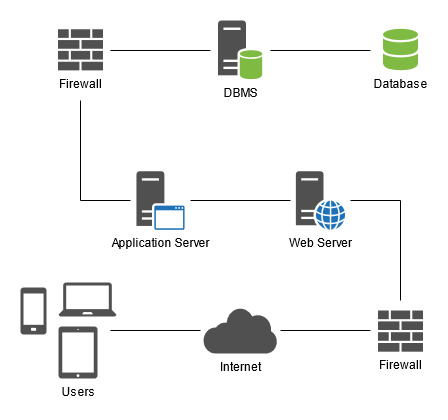
\includegraphics[width=0.95\textwidth]{architecture_overview/physical_architecture_diagram}
\caption{Physical architecture diagram}
\end{figure}

On the client side there is nothing but a browser used to connect to the web server and to dynamically update the \emph{Web App View} when needed (only for minor changes).

The web server, on the other hand, acts as a middleware between the client interface and the system logic, communicating with the user via the standard HTTP protocol, receiving requests and providing adequate responses. To do this, this node also interacts with the application server to submit changes in user data and to request pieces of information needed to generate and update the UI.

Finally, the business logic of the system resides on the application server (\emph{Backend}). This node is able to manage the connection with the DBMS and takes care of carrying out the necessary processing for the correct functioning of the system.

\begin{figure}[H]
\centering
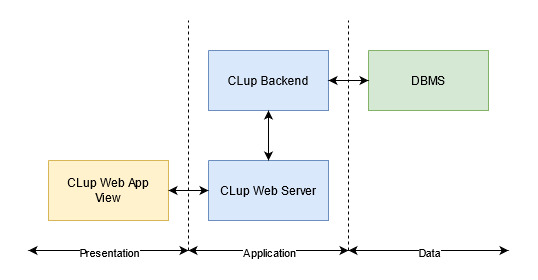
\includegraphics{architecture_overview/high_level_layers}
\caption{High level layers diagram}
\end{figure}

\section{B. Component view}

The following diagrams show the main components of the CLup system and the interfaces through which they interact.\\
For clarity, the first diagram shows a high level view of the components, which are then further explored individually.

The system exposes a RESTful API with multiple public endpoint and resources, some of them require a proper authentication and authorization to be used.

\subsection{B.1. High level component}

\begin{figure}[H]
\centering
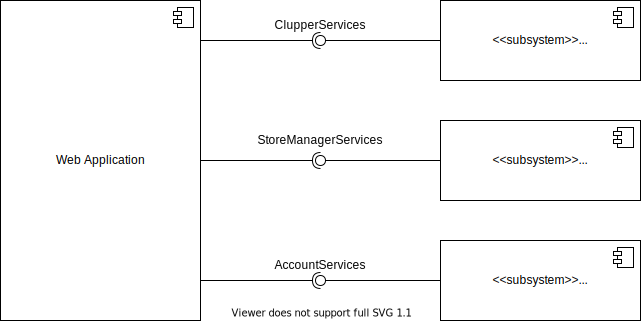
\includegraphics{components_view/high_level_component_diagram}
\caption{High level component diagram}
\end{figure}

The client side consists of a single component that refers to the web application, the only access point to this system.

The server side, on the other end, is made of three subsystems:
\begin{itemize}
\item
    \textbf{Clupper Services}: provides access to the basic services of the application after the login, this services are reserved to the cluppers.
\item
    \textbf{Store Manager Services}: provides access to the managerial services of the application after the login, this services are reserved to the store managers.
\item
    \textbf{Account Services}: provides support to registration, login and logout operations for any type of user.
\end{itemize}

\subsection{B.2. Clupper Services projection}

\begin{figure}[H]
\centering
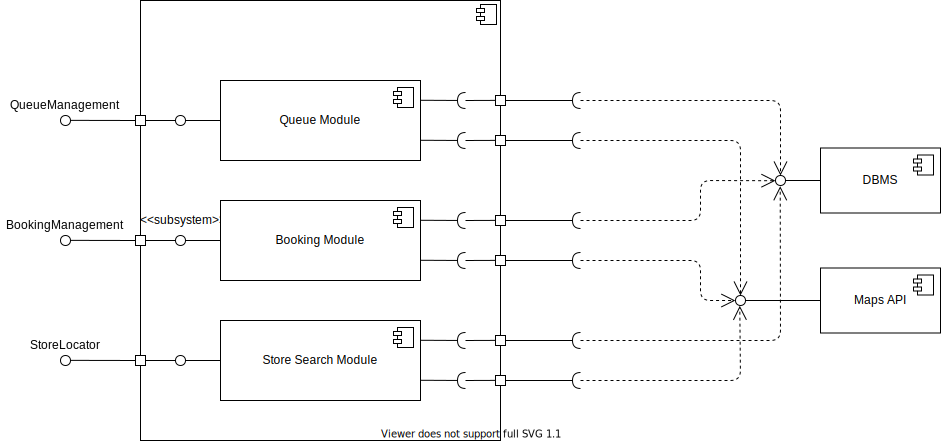
\includegraphics{components_view/clupper_services_projection}
\caption{Clupper Services projection diagram}
\end{figure}

The Clupper Services subsystem contains three components:
\begin{itemize}
\item
    \textbf{Queue Module}: offers the \emph{QueueManagement} interface to handle all the operations related to the join the queue function.
\item
    \textbf{Booking Module}: offers the \emph{BookingManagement} interface to handle all the operations related to the book a visit function.
\item
    \textbf{Store Locator}: offers the \emph{StoreLocator} interface that allows the client to retrieve information about the stores.
\end{itemize}
In order to fulfill their goals, these components need to communicate with the DBMS and the Maps API through the corresponding interfaces.

\subsection{B.3. Store Manager Services projection}

\begin{figure}[H]
\centering
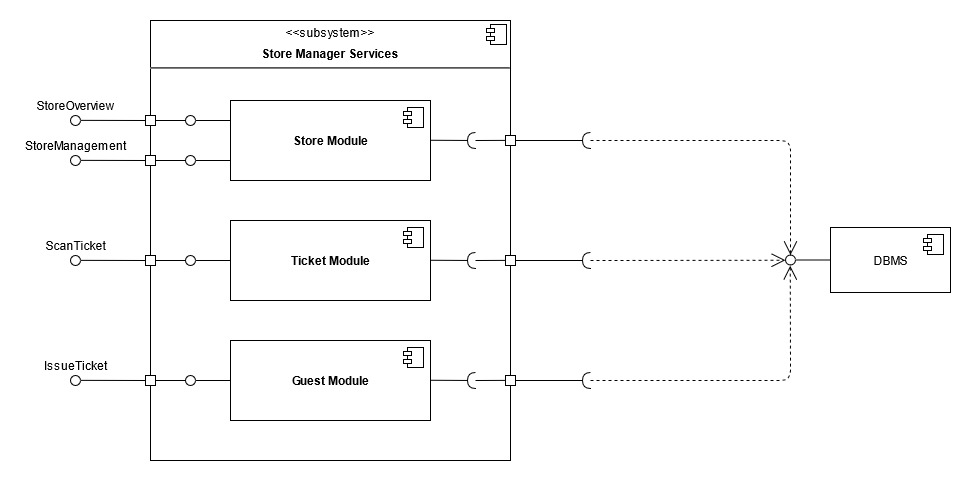
\includegraphics{components_view/store_manager_services_projection}
\caption{Store Manager Services projection diagram}
\end{figure}

The Store Manager Services subsystem contains three components:
\begin{itemize}
\item
    \textbf{Store Module}: offers the \emph{StoreOverview} and the
    \emph{StoreManagement} interfaces used to receive store status updates and to edit the store maximum capacity respectively.
\item
    \textbf{Ticket Module}: offers the \emph{ScanTicket} interface to receive feedback on scanned tickets.
\item
    \textbf{Guest Module}: offers the \emph{IssueTicket} interface to request a queue ticket for a guest.
\end{itemize}

In order to fulfill their goals, these components need to communicate with the DBMS.

FIXME \emph{[Camera, Printer external interfaces?]}

\subsection{B.4. Account Services projection}

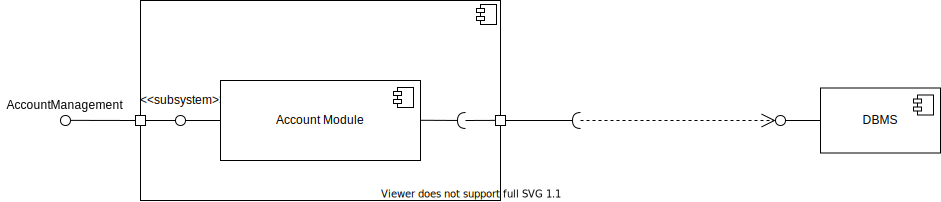
\includegraphics{components_view/account_services_projection}
The Account Services subsystem contains one component:
\begin{itemize}
\item
    \textbf{Account Module}: offers the \emph{AccountManagement} interface to handle the operations of register, login and logout.
\end{itemize}

In order to fulfill its goals, this component needs to communicate with the DBMS.

\subsection{B.5. ER diagram}

The following diagram provides a graphical representation of the conceptual model of the database.

\begin{figure}[H]
\centering
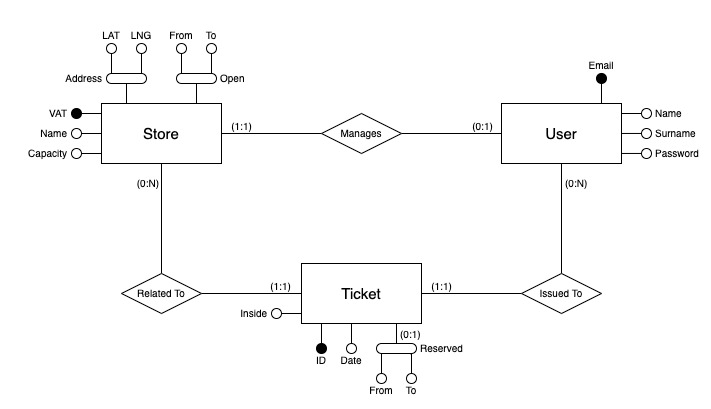
\includegraphics{components_view/er_diagram}
\caption{Entity-relationship diagram}
\end{figure}

\section{C. Deployment view}

\begin{figure}[H]
\centering
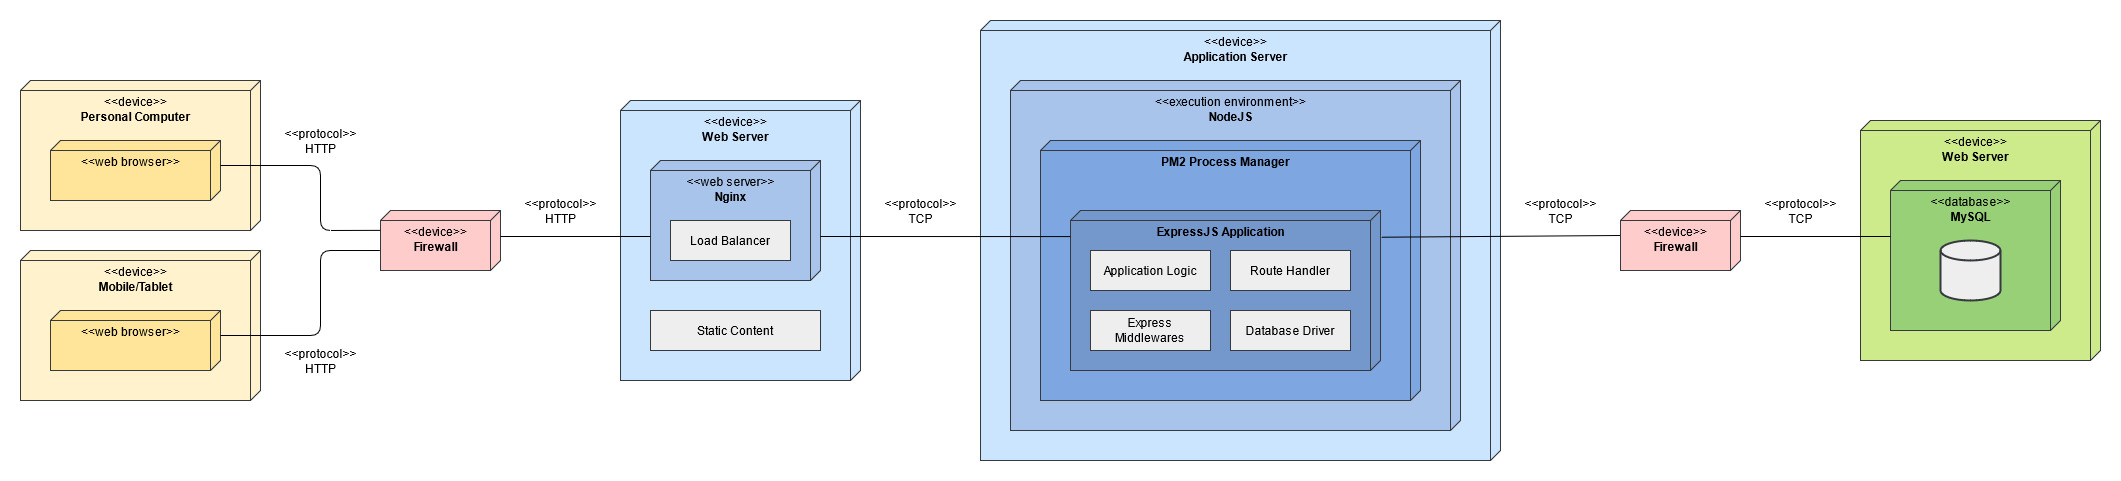
\includegraphics{deployment_view/deployment_diagram}
\caption{Deployment diagram}
\end{figure}

The system architecture is divided in 4 tiers:
\begin{itemize}
\item
    The first tier is the \emph{client tier}: it is composed by any device capable of rendering a web page (smartphones, tablets, PC). It communicates with the web tier through the HTTP protocol.
\item
    The \emph{web tier} contains the web server implemented with Nginx platform. This tier is provided with a load balancer to distribute the load between the multiple instances of the application tier.
\item
    The third tier is the \emph{application tier}. The CLup backend is built on an Express application which is managed by a docker-like process manager to spawn multiple instances. The execution environment is the NodeJS runtime.
\item
    The \emph{data tier} is the fourth tier composed by the Database server.
\end{itemize}

\subsection{C.1. Recommended implementation}

\begin{itemize}
\item
    \textbf{Client tier}: The client web browser may be an arbitrary one,the only constraint is that it must be recent enough to render HTML5 and CSS3 web pages and execute Javascript.
\item
    \textbf{Web tier}: The web tier must be implemented with Nginx web server. A load balancer is also needed to distribute the load between the multiple instances of the application. It is strongly recommended to setup the load balancer to use a Round Robin algorithm to distribute the load, to avoid overloading a single application instance.
\item
    \textbf{Application tier}: The runtime engine where the backend lives is NodeJS and a docker-like process manager (PM2) is used to spawn multiple instances of the application, which uses ExpressJS to expose services.
\item
    \textbf{Data tier}: The database is relational and is implemented using MySQL.
\end{itemize}

\section{D. Runtime view}

The following sequence diagrams describe the interactions between the main components of the product when utilizing the most common features.\\
This is still a high-level description of the actual interactions so that they can be slightly modified during the development process.

\subsection{D.1. User login}

\begin{figure}[H]
\centering
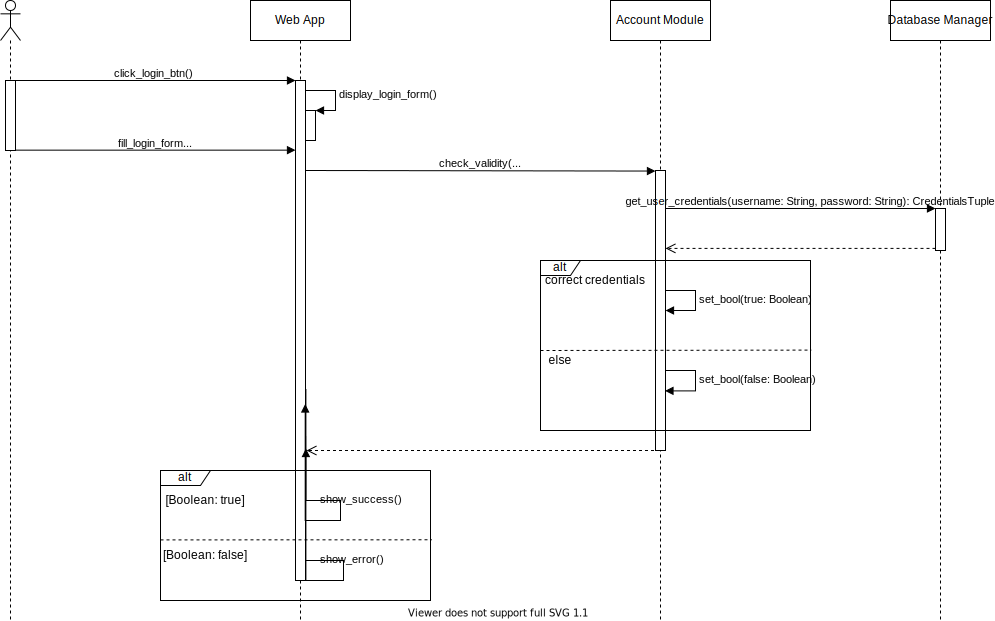
\includegraphics{sequence_diagrams/user_login_sequence_diagram}
\caption{User login sequence diagram}
\end{figure}

\subsection{D.2. User book a visit}

\begin{figure}[H]
\centering
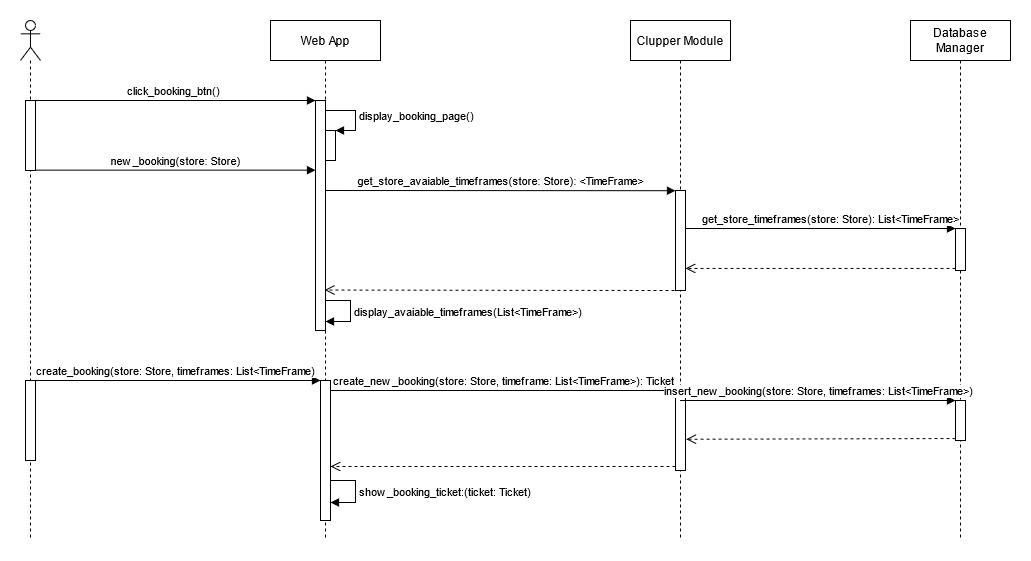
\includegraphics{sequence_diagrams/clupper_booking_sequence_diagram}
\caption{User book a visit sequence diagram}
\end{figure}

\subsection{D.3. Store manager scan ticket}

\begin{figure}[H]
\centering
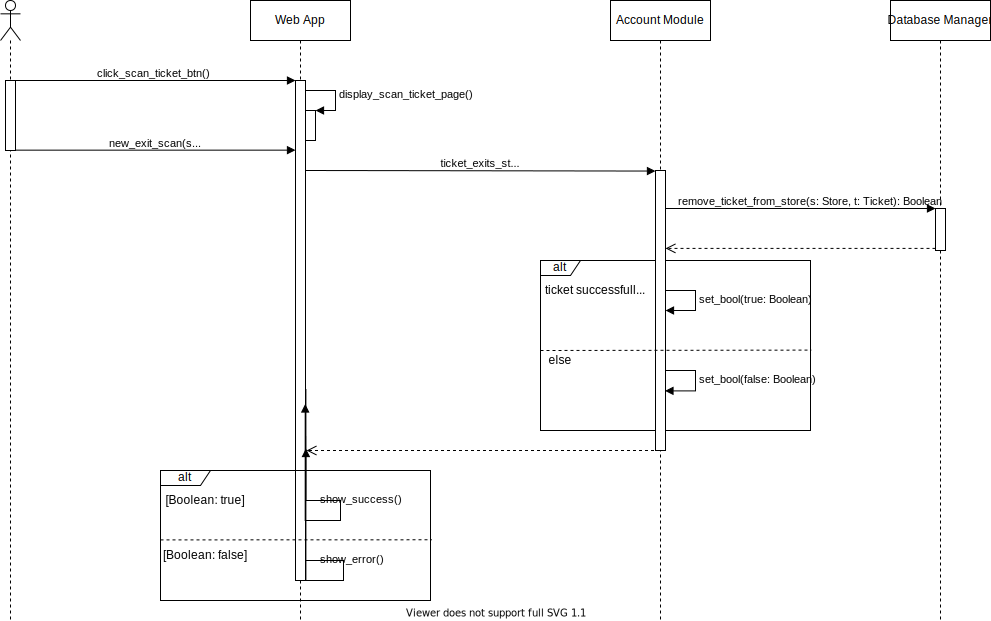
\includegraphics{sequence_diagrams/store_manager_scan_sequence_diagram}
\caption{Store manager scan ticket sequence diagram}
\end{figure}

\section{E. Component interface}

These diagrams show the main methods provided by each component:
\begin{itemize}
\item
    The \emph{ClupperServices} interface provides every method the clupper could need to access every functionality of the application. In particular there are methods to join the queue, book a visit and find stores.
\item
    Like ClupperServices, \emph{StoreManagerServices} provides all methods a store manager needs to manage the store. In fact, he's allowed to edit the store capacity, check the number of customers inside, in line and with a reservation and lend out physical tickets to guests.
\item
    \emph{AccountServices} is an interface accessible by both users and visitors. It let's the users login and logout and allows the registration of new cluppers or store managers.
\end{itemize}

\subsection{E.1. ClupperServices interface}

\begin{figure}[H]
\centering
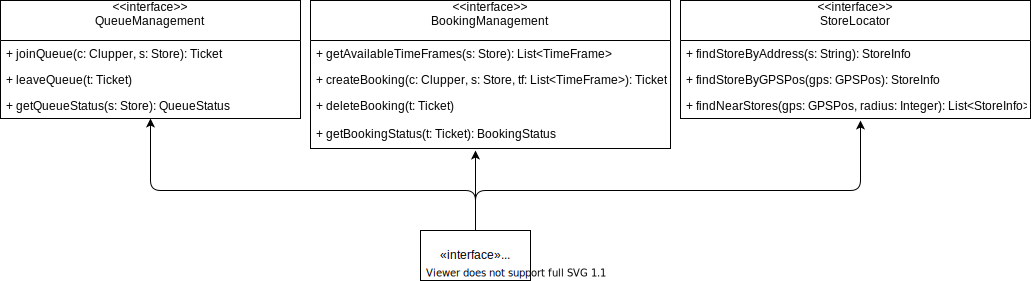
\includegraphics[width=0.93\textwidth]{component_interface_diagrams/clupper_component_interface_diagram}
\caption{ClupperServices interface diagram}
\end{figure}

\subsection{E.2. StoreManagerServices interface}

\begin{figure}[H]
\centering
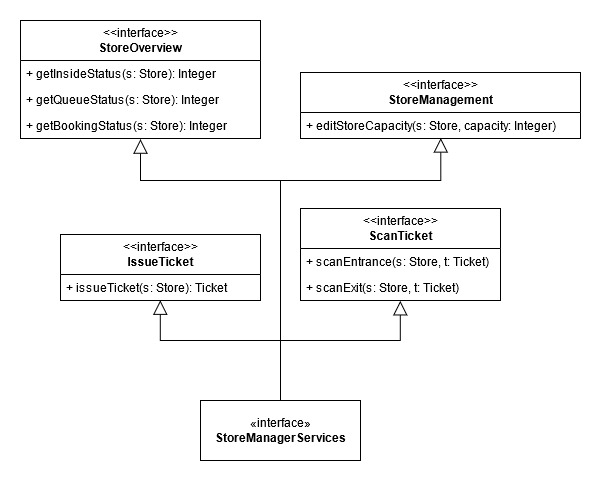
\includegraphics[width=0.93\textwidth]{component_interface_diagrams/store_manager_component_interface_diagram}
\caption{StoreManagerServices interface diagram}
\end{figure}

\subsection{E.3. AccountServices interface}

\begin{figure}[H]
\centering
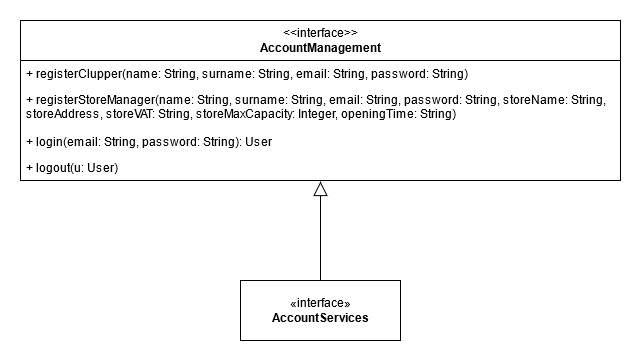
\includegraphics[width=0.93\textwidth]{component_interface_diagrams/account_management_component_interface_diagram}
\caption{AccountServices interface diagram}
\end{figure}

\section{F. Selected architectural styles and patterns}
FIXME \emph{[Update]}

\subsection{F.1. MVC pattern}

The Model-View-Controller pattern is used in order to obtain a clear division between the internal representation of information, the way in which that information is presented to the user and the business logic of the system.\\
This is one of the most common and effective ways to drastically reduce the level of coupling between the various parts of the system.

\subsection{F.2. RESTful API with JSON}

The application layer of the system offers a set of services that each client is able to address via HTTP protocol.\\
As prescribed by the REST principles, for each incoming request the server provides a response that can also include a JSON representation of one or more objects.

\subsection{F.3. Other design patterns}

\begin{itemize}
    \item \textbf{Facade pattern}: supplies a single interface to a set of interfaces within the system.
    \item \textbf{Factory pattern}: exposes a method for creating objects, allowing subclasses to control the actual creation process.
    \item \textbf{Observer pattern}: notifies the subscribed objects when the state of the observed object is updated.
    \item \textbf{Proxy pattern}: allows object level access control by acting as a pass through entity or a placeholder object.
    \item \textbf{Singleton pattern}: provides a single instance of a class that is able to coordinate all the actions across the system.
\end{itemize}

\section{G. Other design decisions}

\subsection{G.1. Maps API}

To implement some of the system functions (which require GPS information), the use of an external service is unavoidable.\\
When dealing with third party software it is important to be able to trust its source, for this reason CLup will use the API offered by Google Maps.\\
In particular, as this system will be developed as a web application, the \emph{Google Maps Javascript API} is recommended.

\chapter{3. User interface design}

\section{A. UI mockups}

The following mockups (already presented in section \emph{3.A.1. User interfaces} of the RASD) provide an idea of how the web application offered by CLup will look like.

Since the main devices that will use the system are portable, a mobile-first approach is recommended in the UI development, however, the client view must be designed responsively to best fit any screen size.

\begin{figure}[H]
    \centering
    \begin{subfigure}[t]{0.28\textwidth} 
        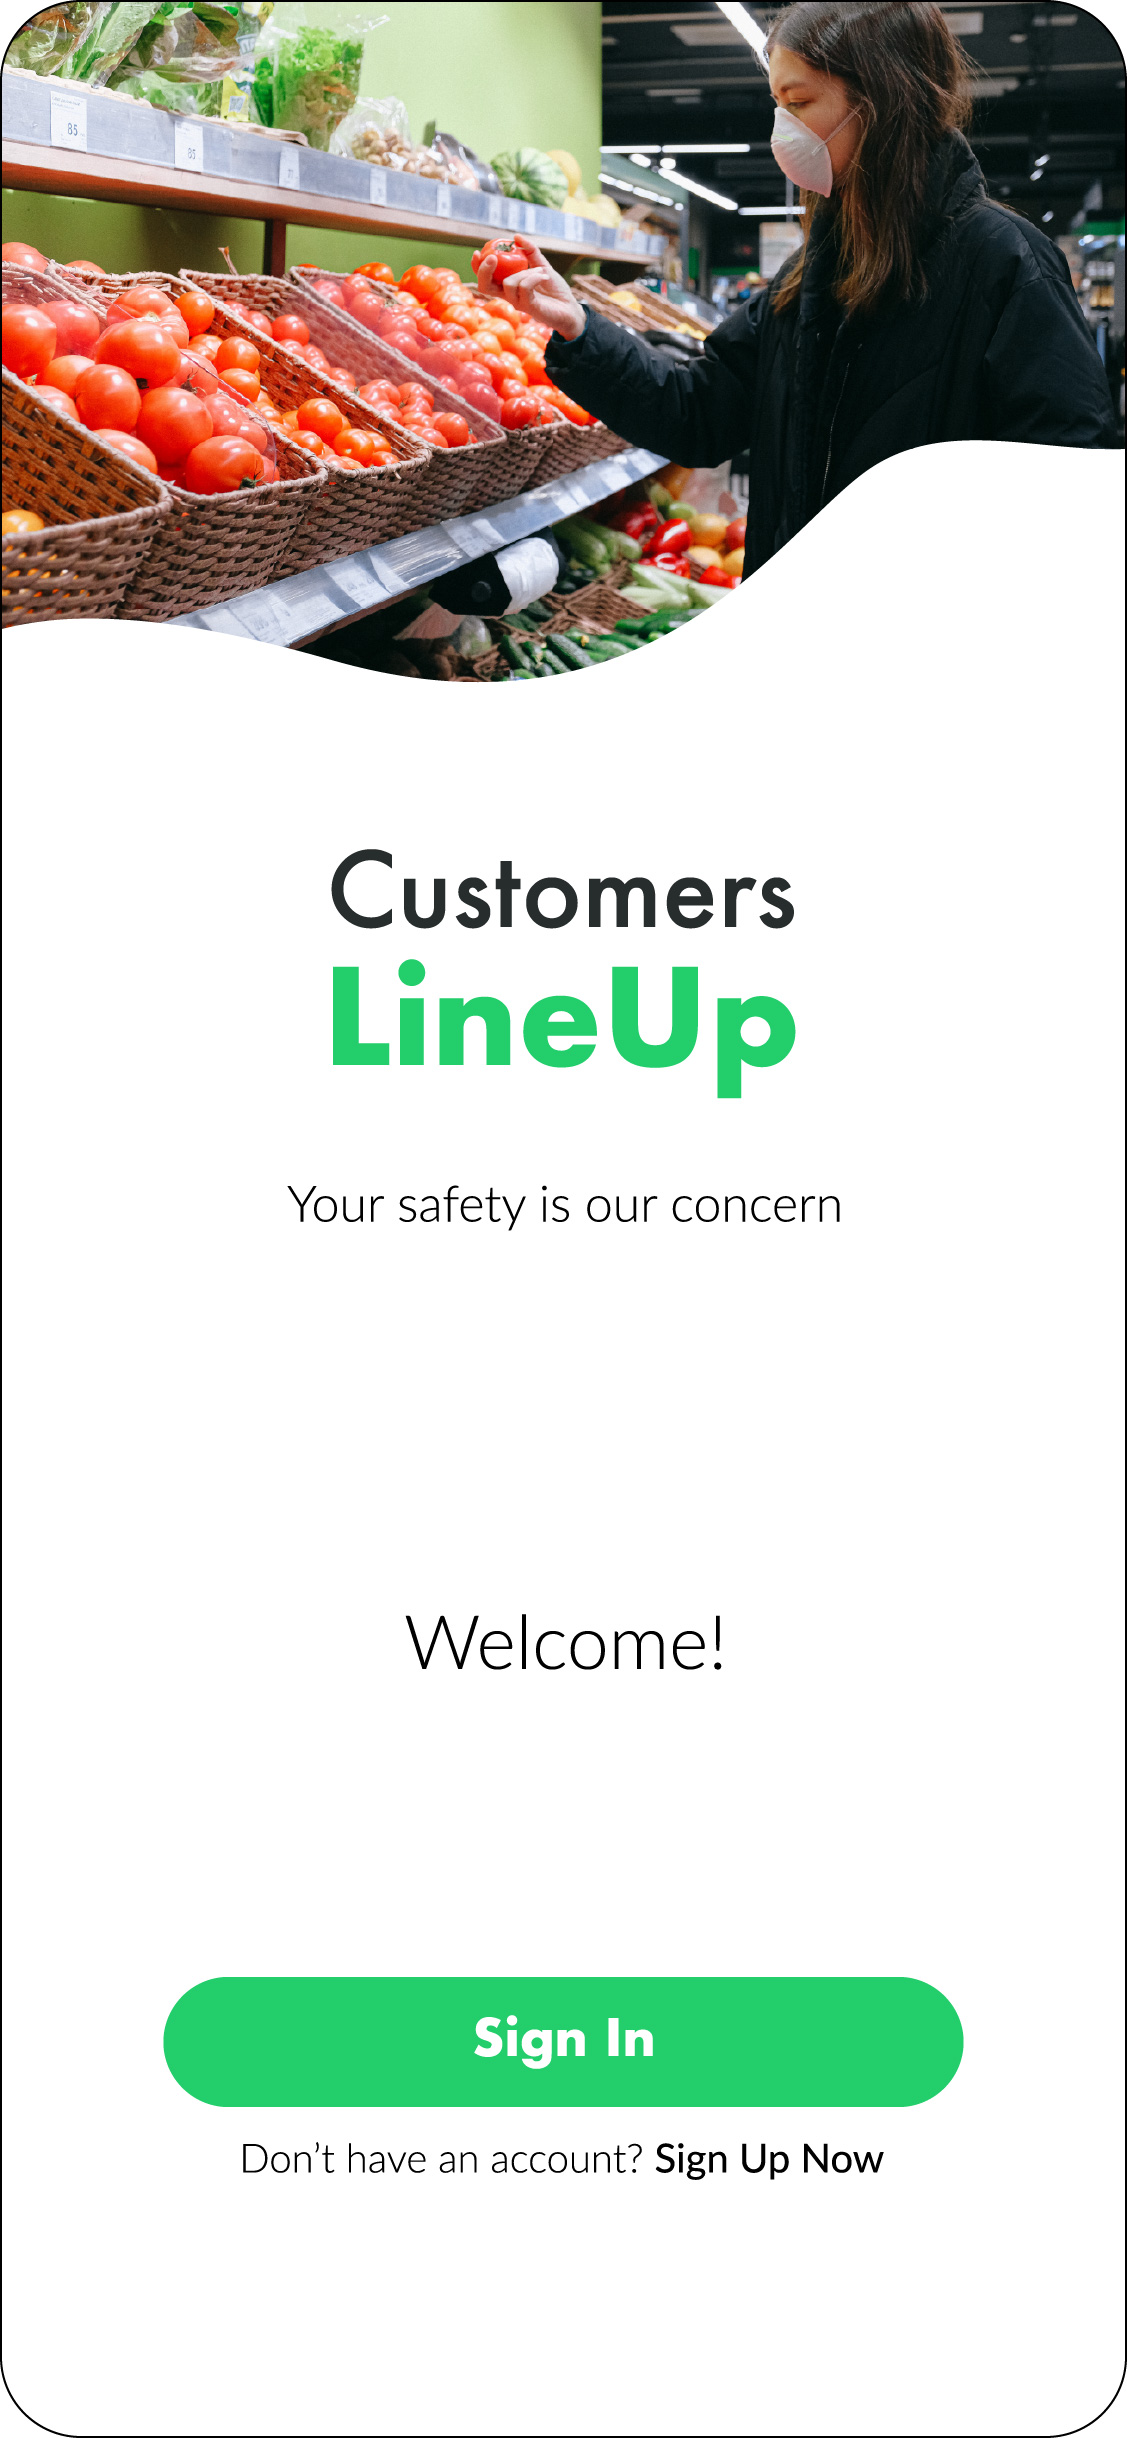
\includegraphics{../mockups/home}
        \caption*{Home page}
    \end{subfigure}
    \quad
    \begin{subfigure}[t]{0.28\textwidth} 
        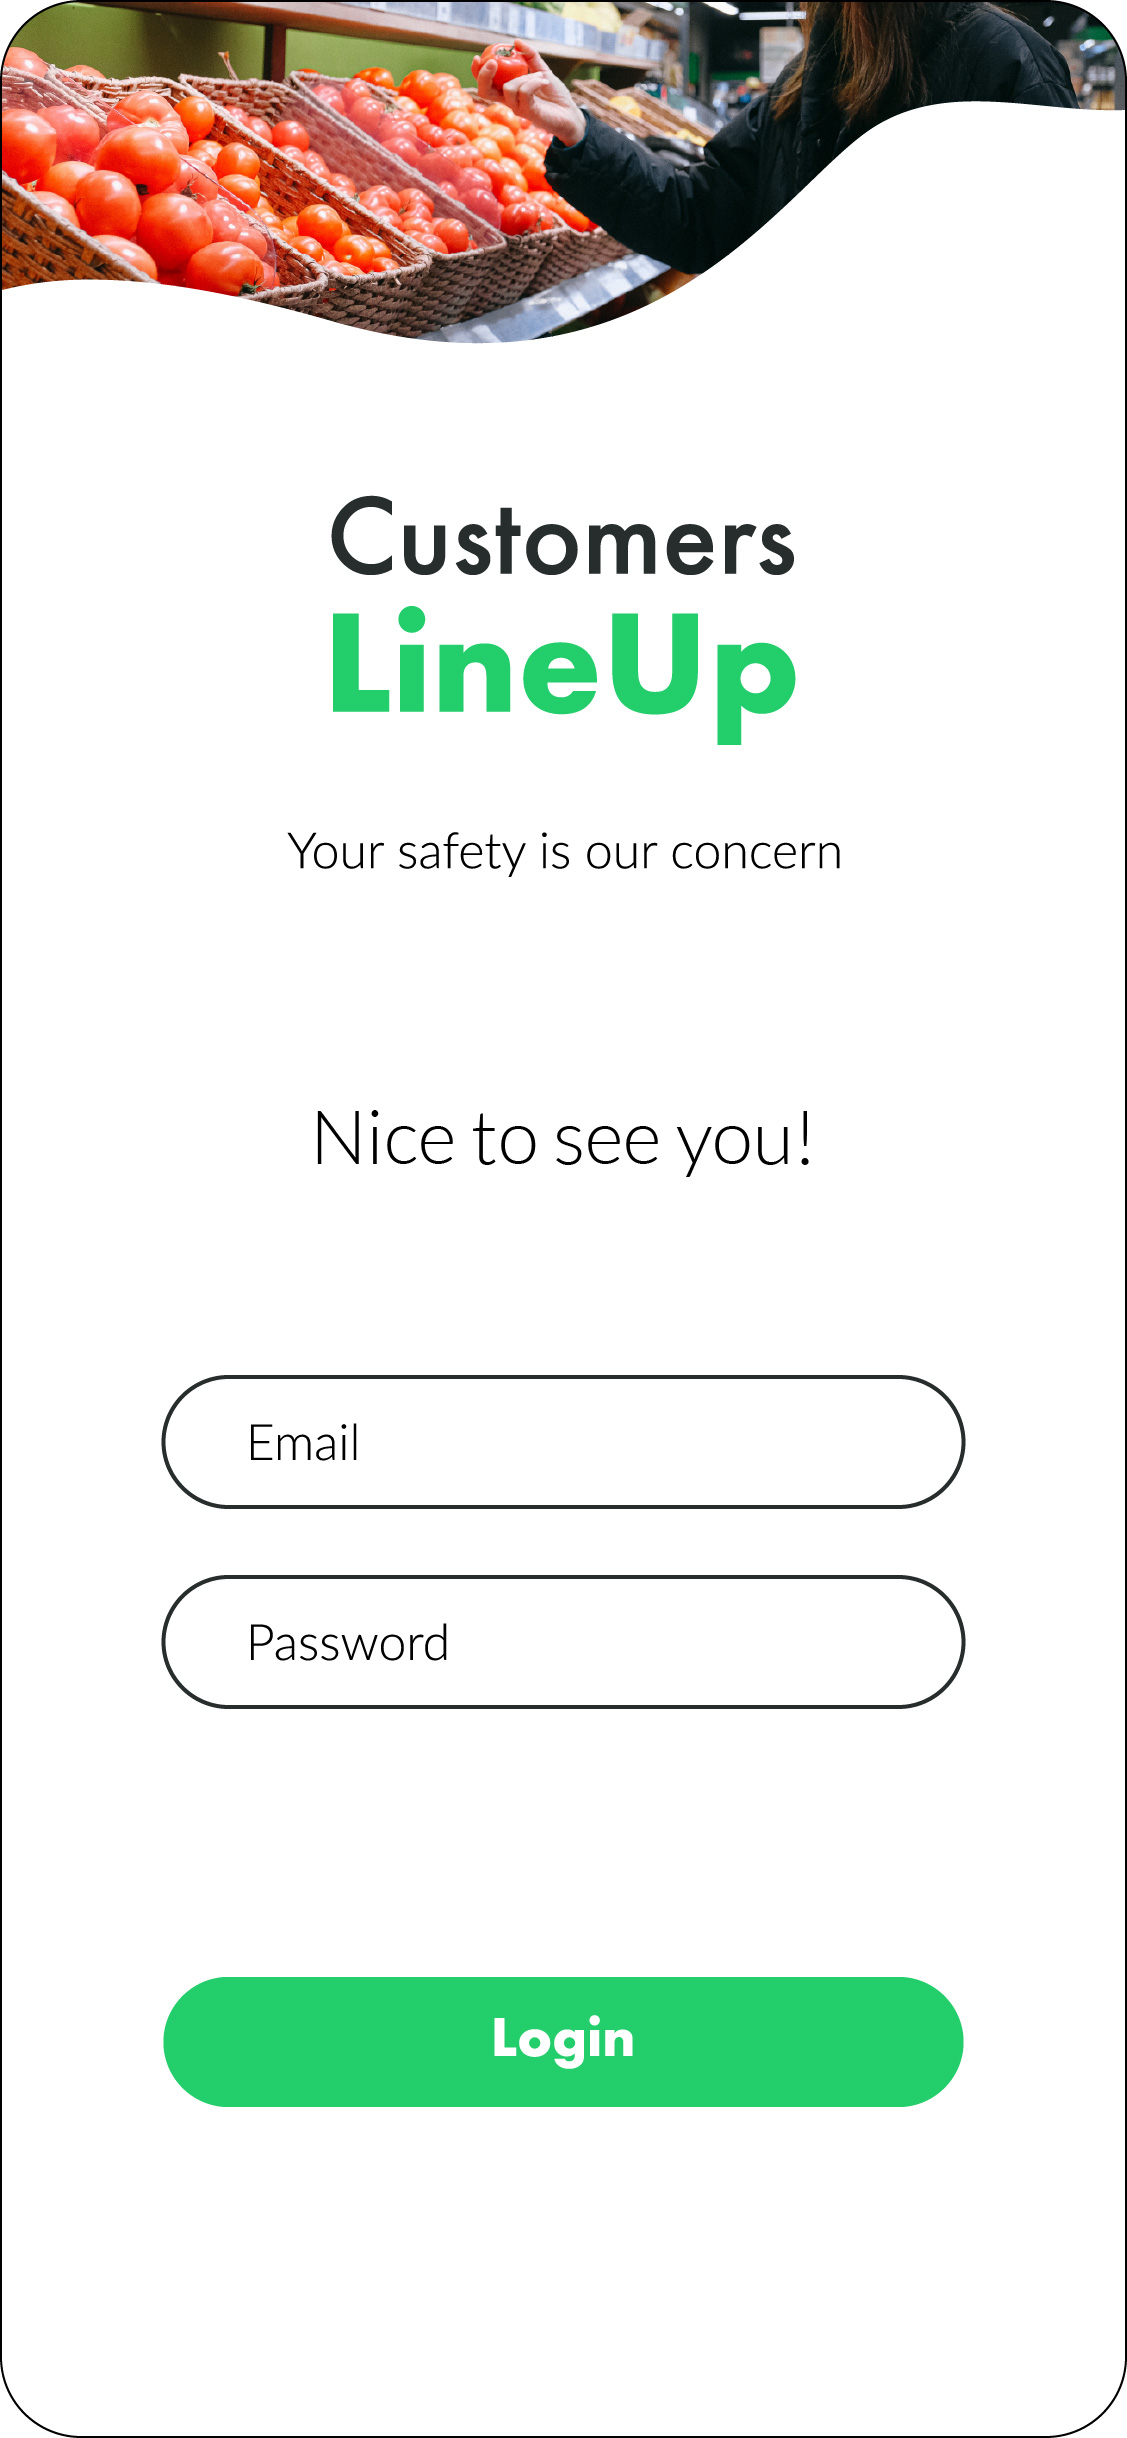
\includegraphics{../mockups/sign_in}
        \caption*{Sign in page}
    \end{subfigure}
    \quad
    \begin{subfigure}[t]{0.28\textwidth} 
        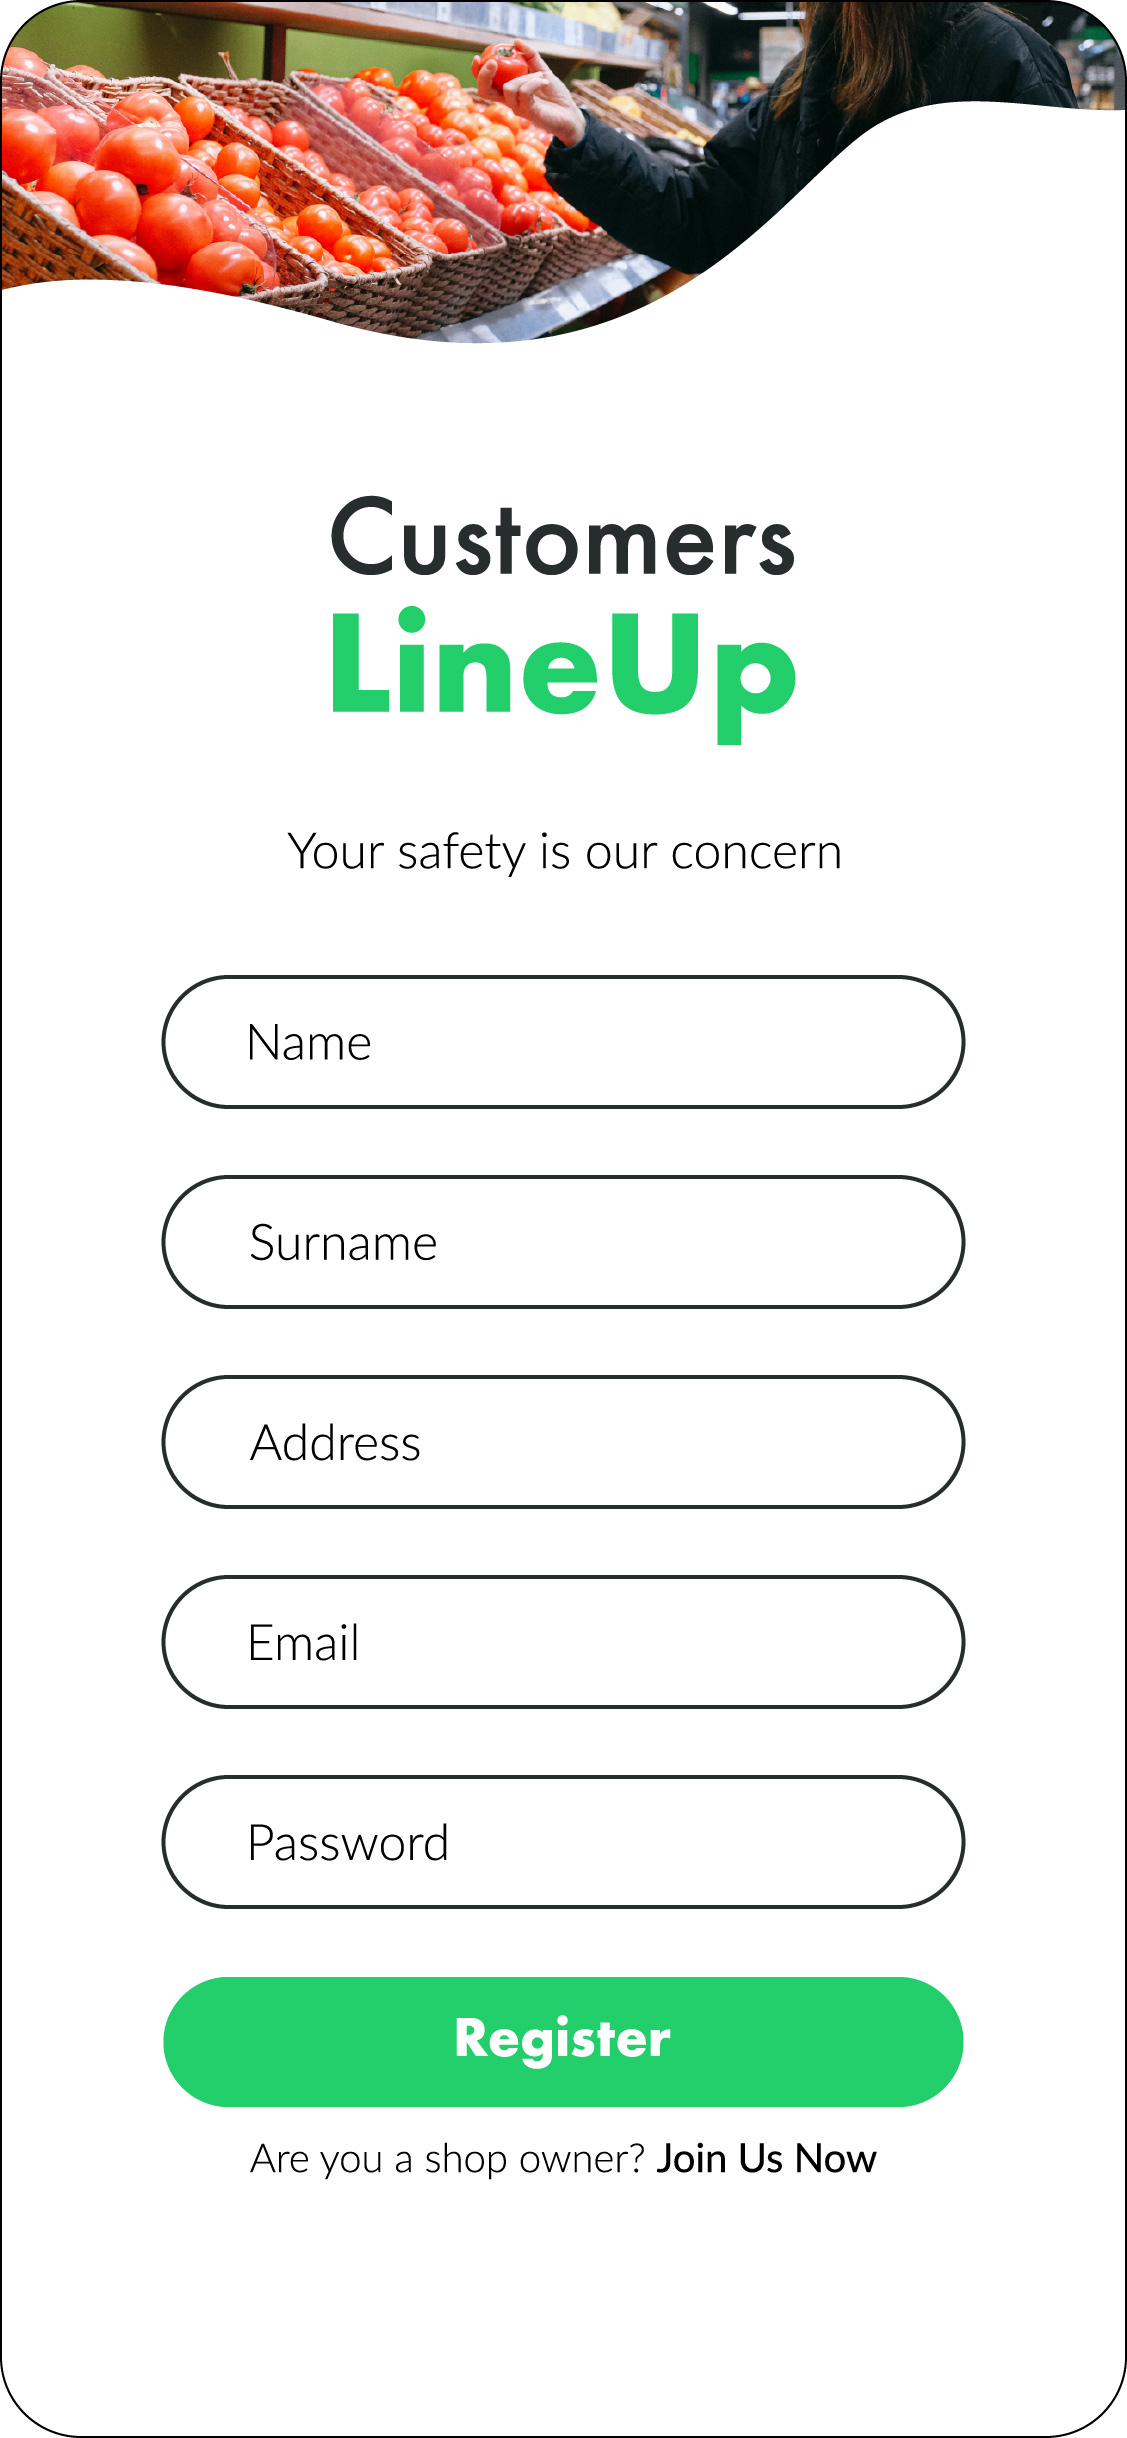
\includegraphics{../mockups/sign_up}
        \caption*{Sign up page}
    \end{subfigure}
\end{figure}

\begin{figure}[H]
    \centering
    \begin{subfigure}[t]{0.28\textwidth} 
        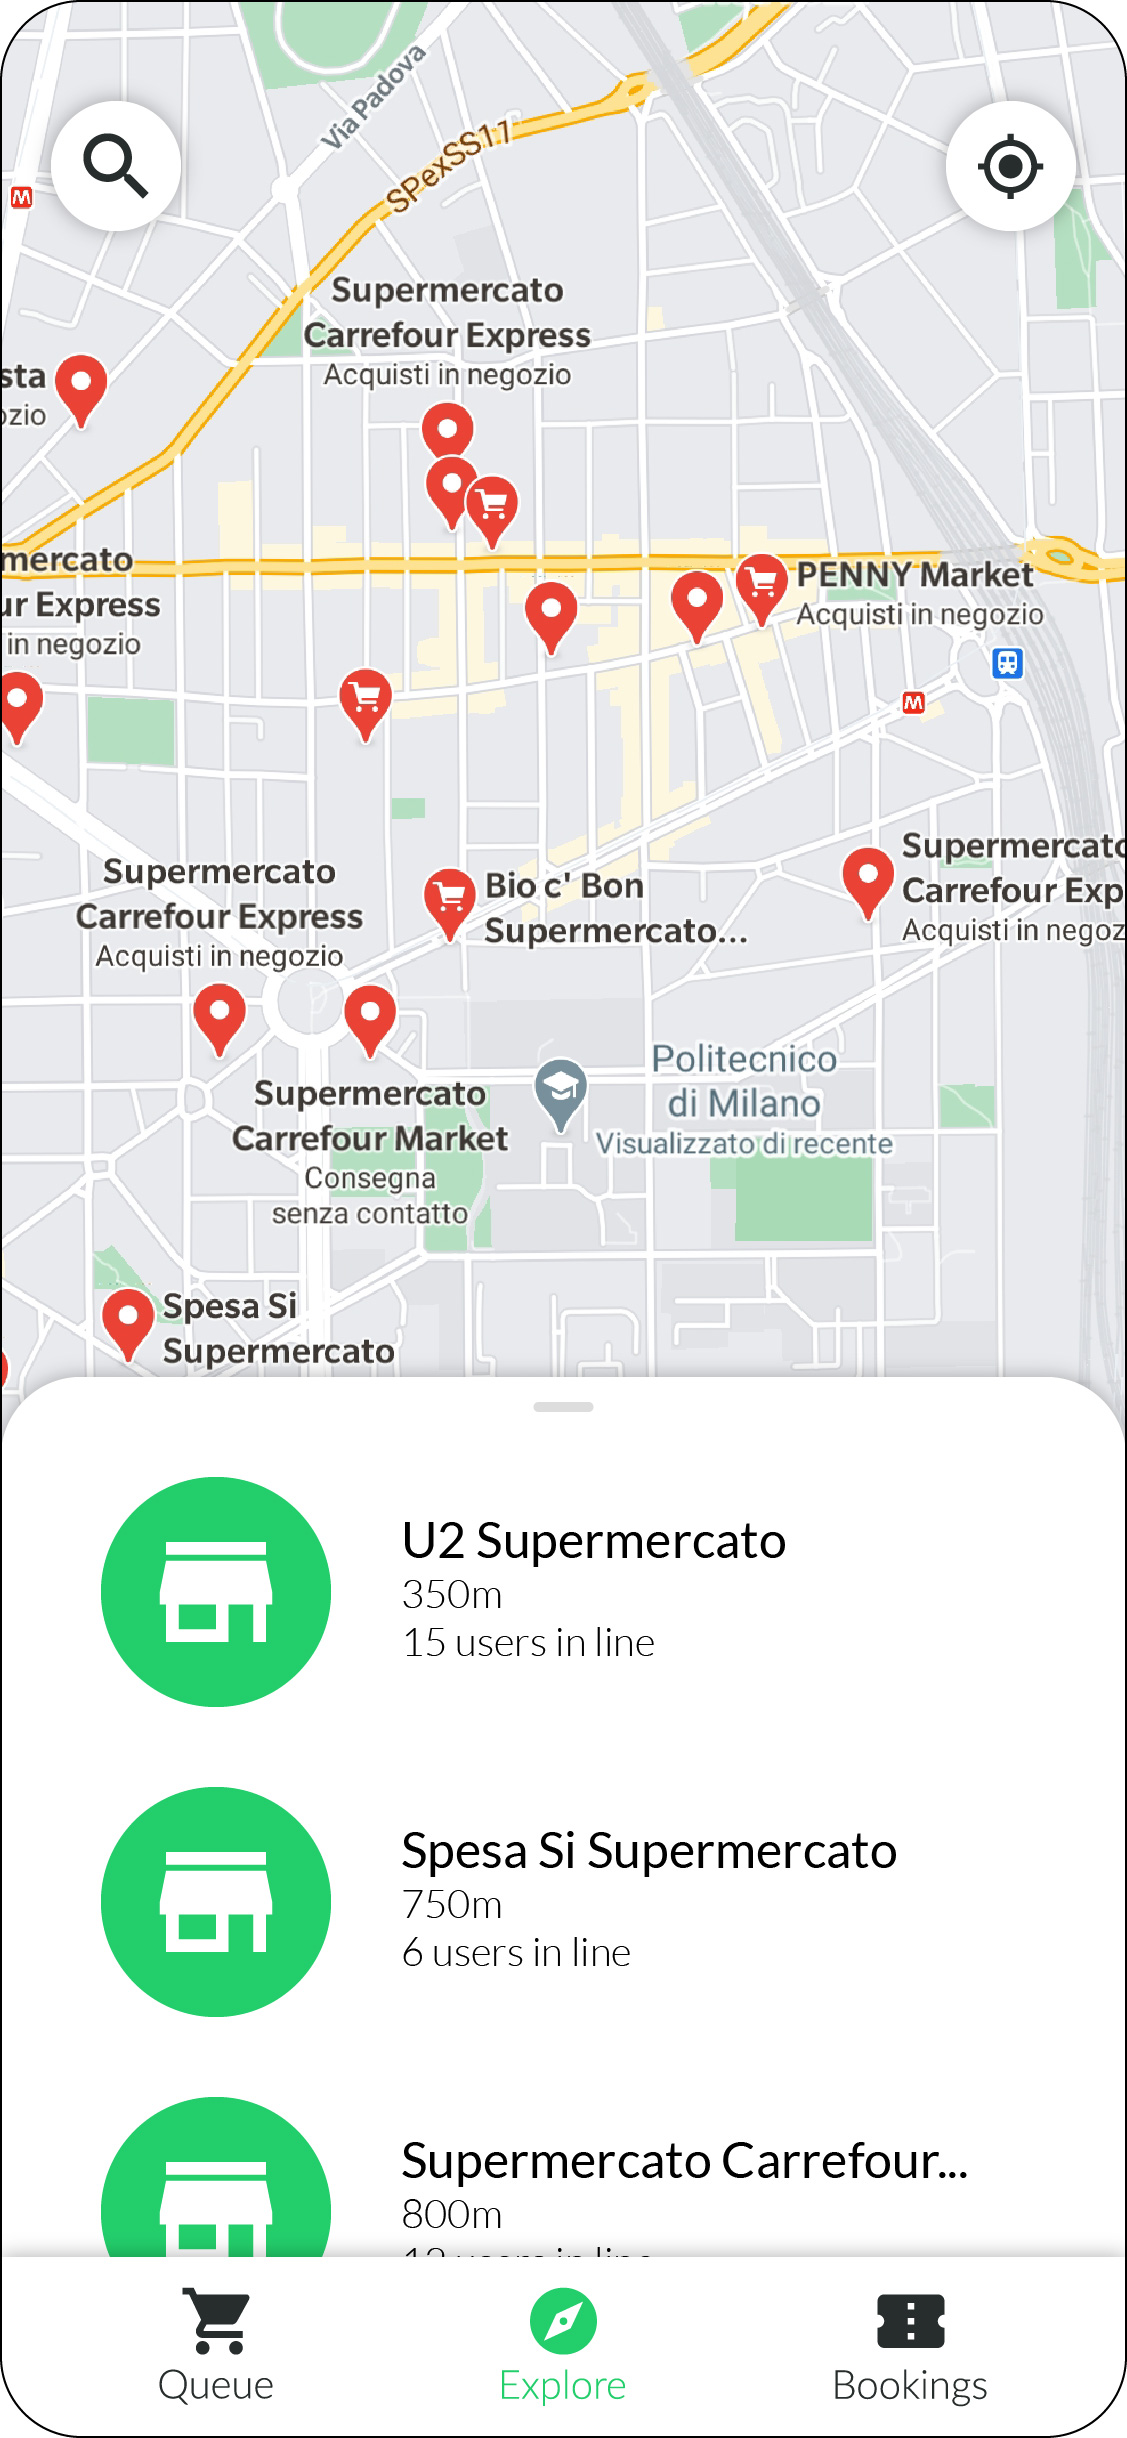
\includegraphics{../mockups/map}
        \caption*{Map page}
    \end{subfigure}
    \quad
    \begin{subfigure}[t]{0.28\textwidth} 
        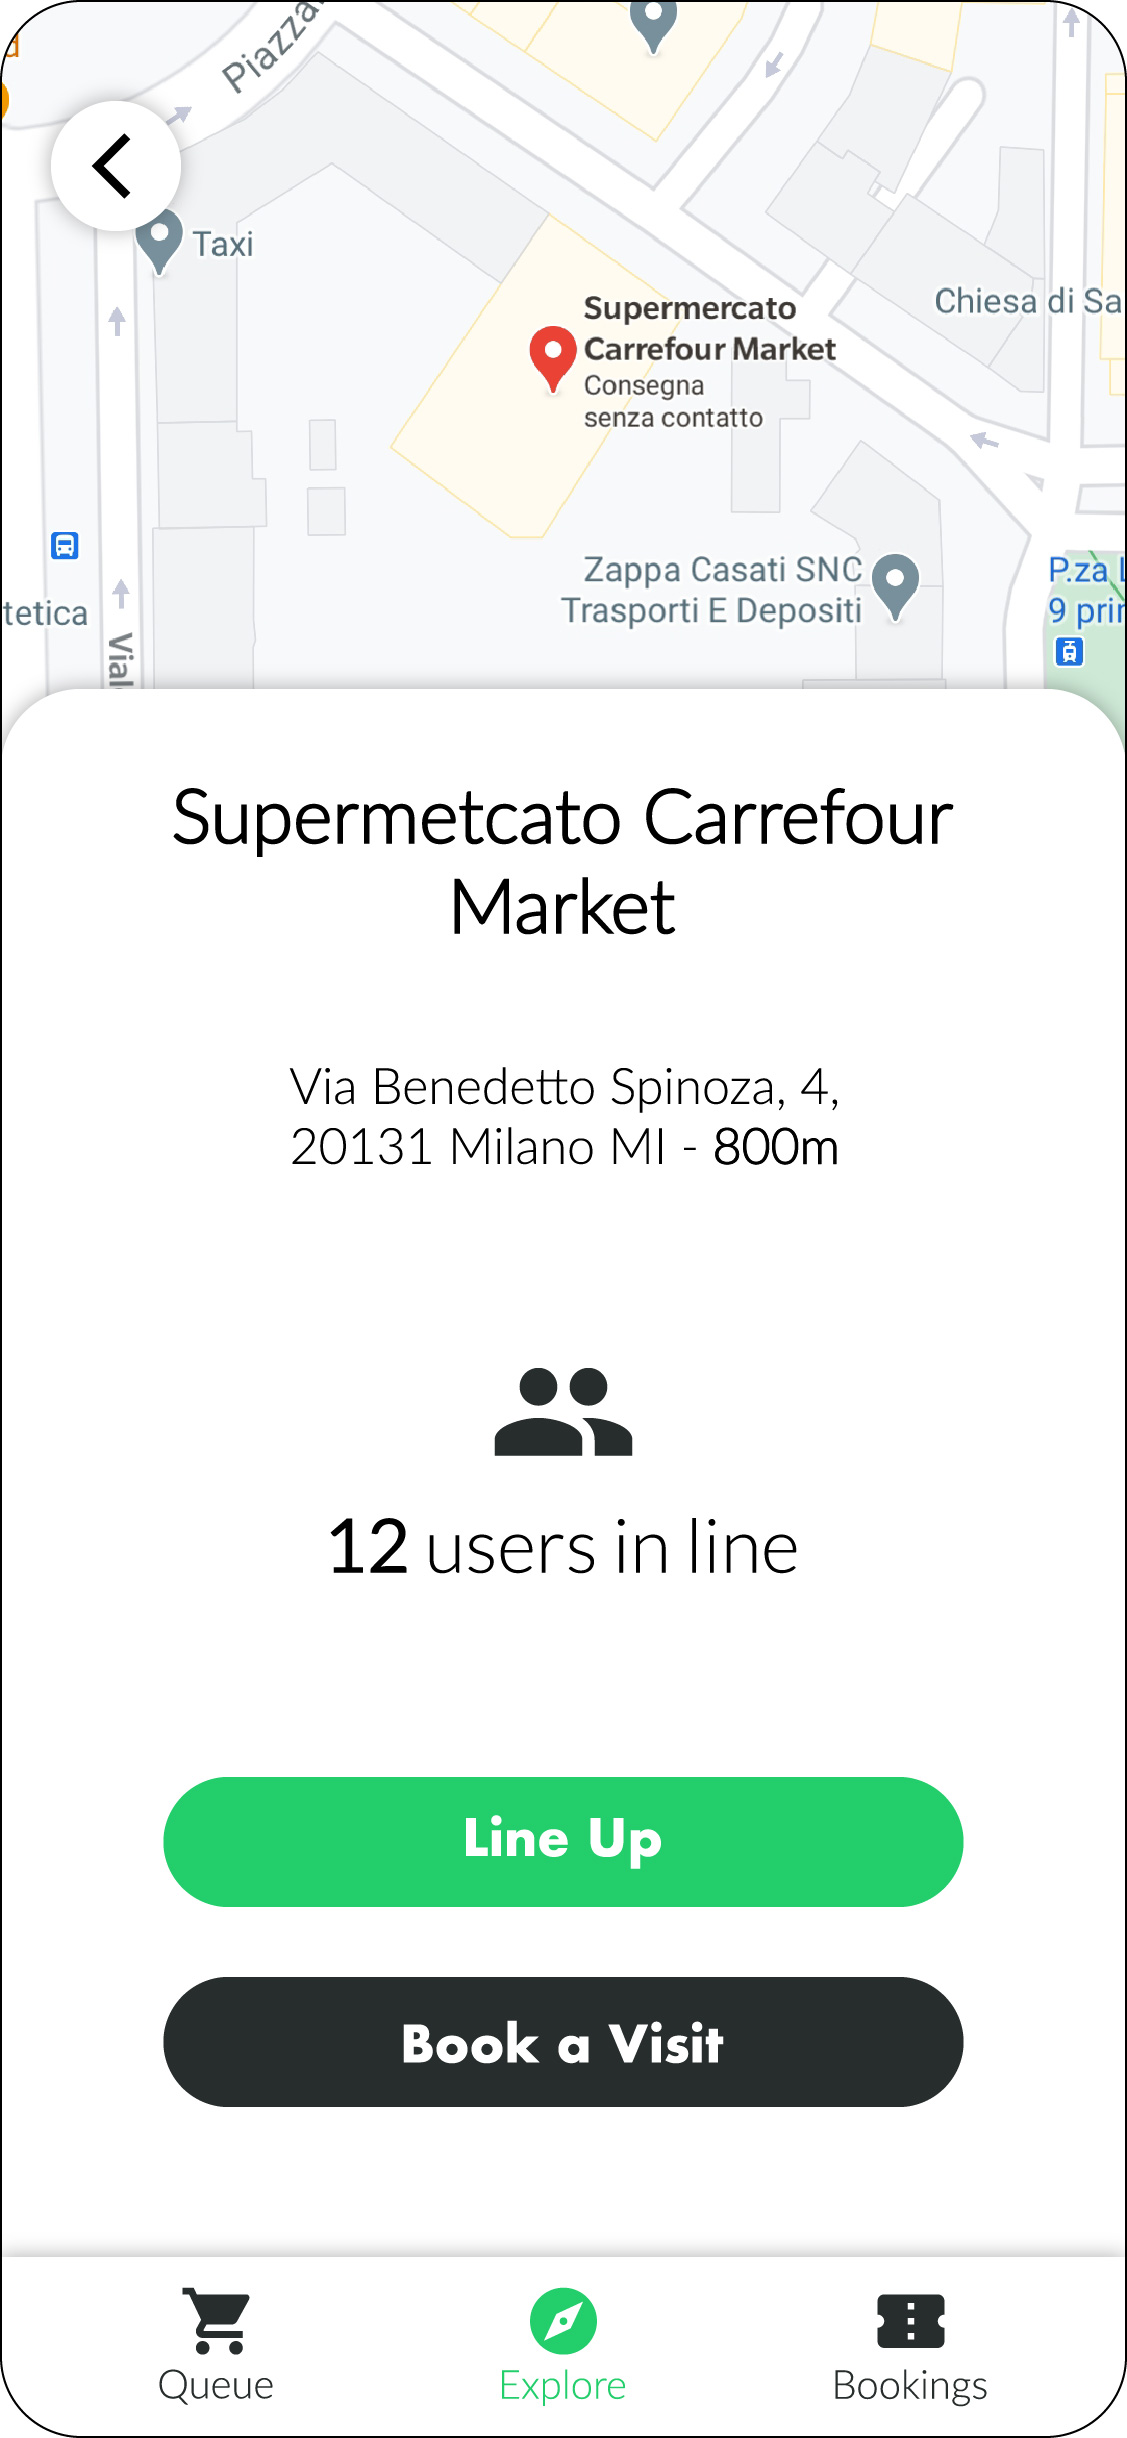
\includegraphics{../mockups/store}
        \caption*{Store page}
    \end{subfigure}
    \quad
    \begin{subfigure}[t]{0.28\textwidth} 
        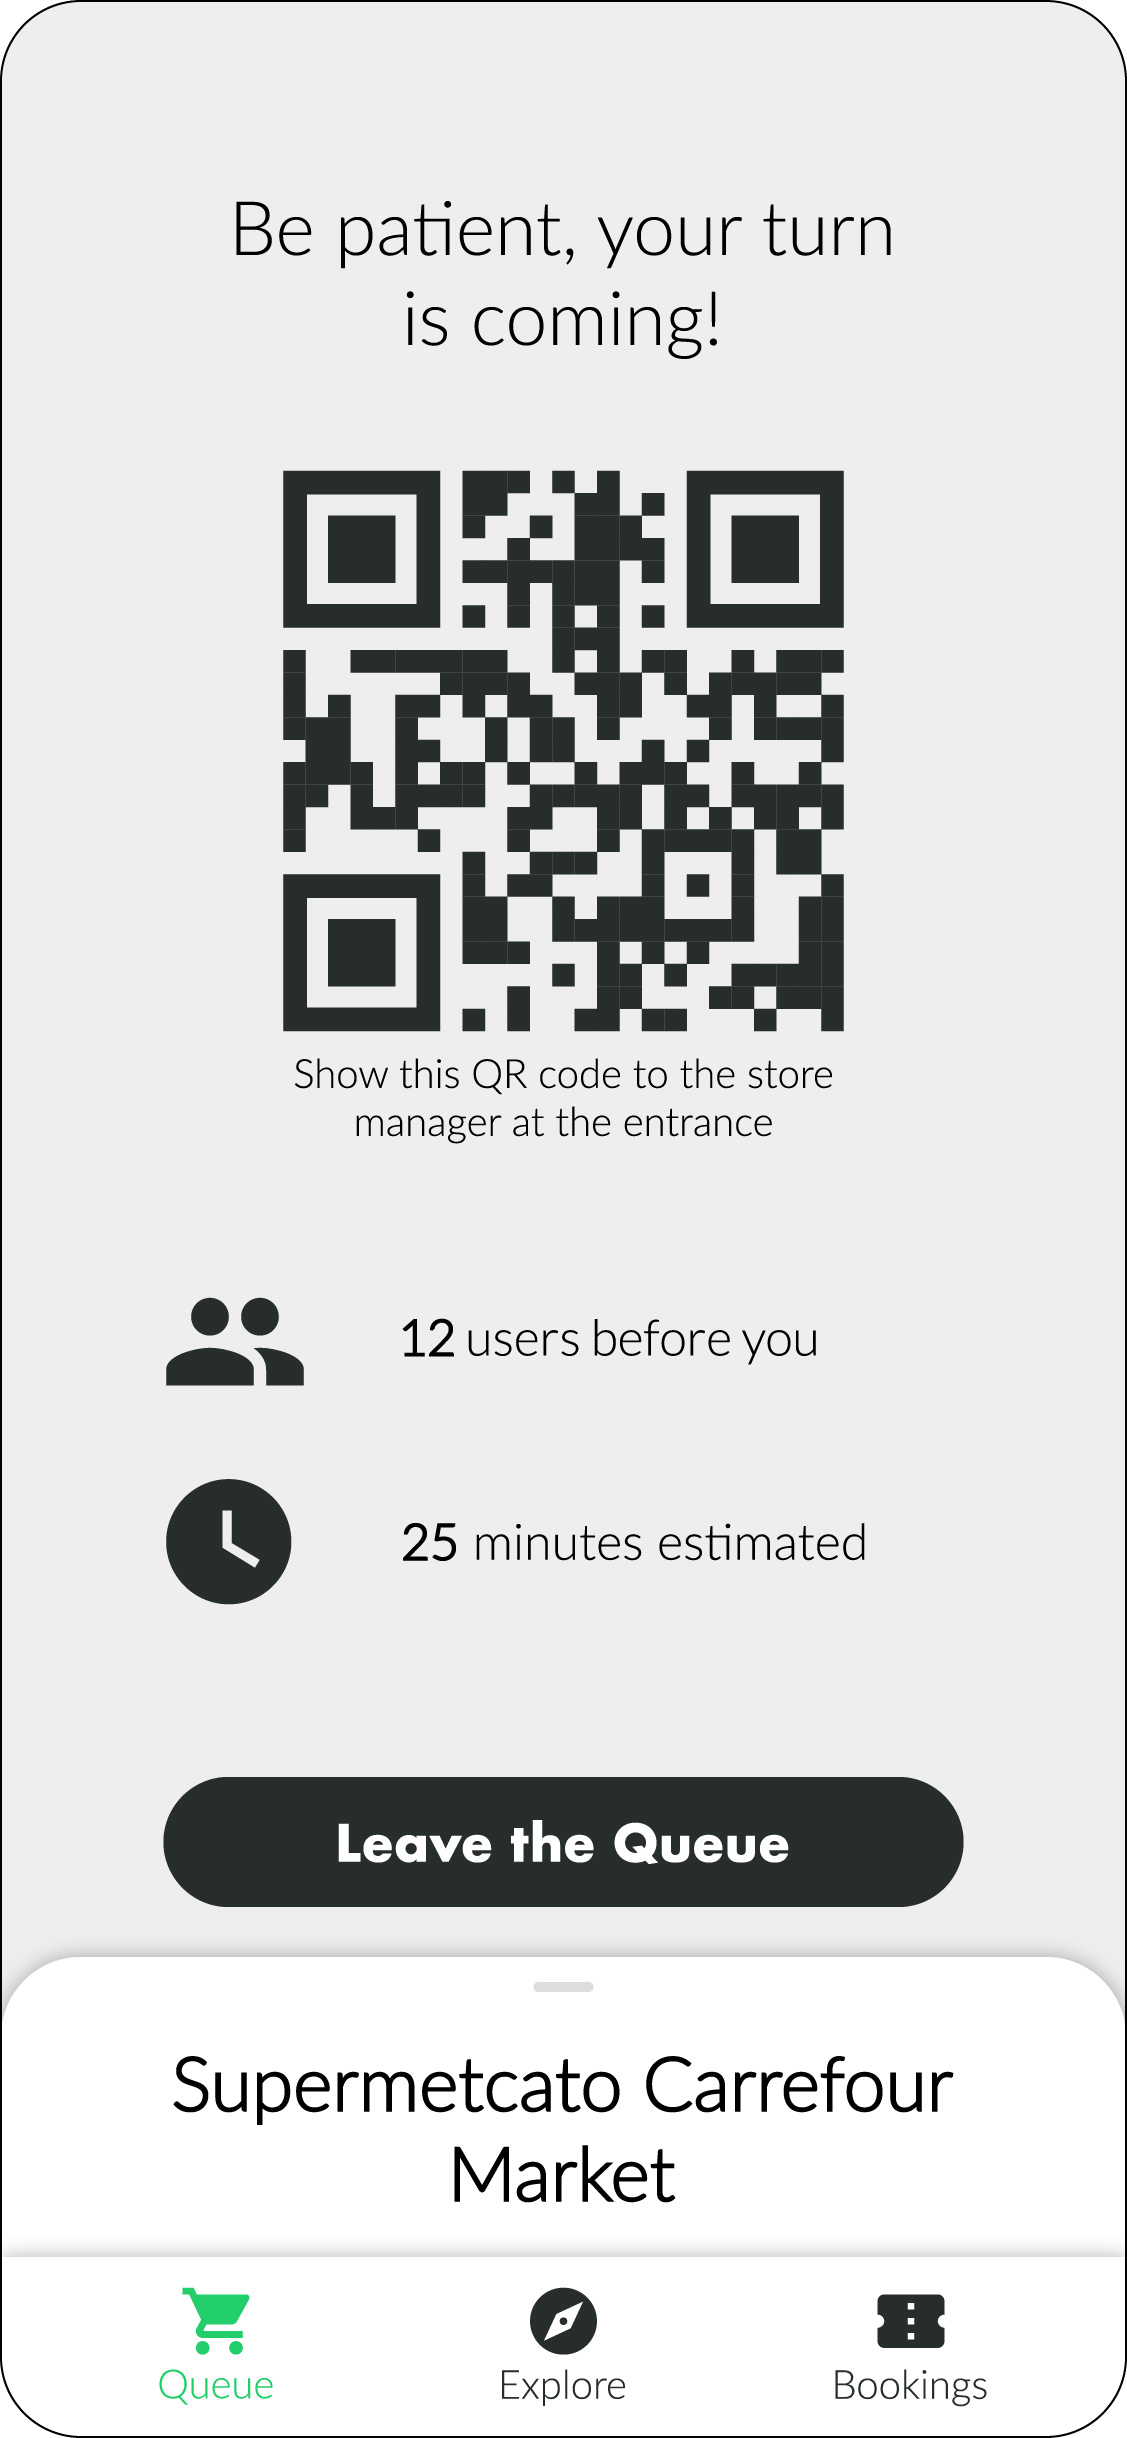
\includegraphics{../mockups/queue}
        \caption*{Queue page}
    \end{subfigure}
\end{figure}

\begin{figure}[H]
    \centering
    \begin{subfigure}[t]{0.28\textwidth} 
        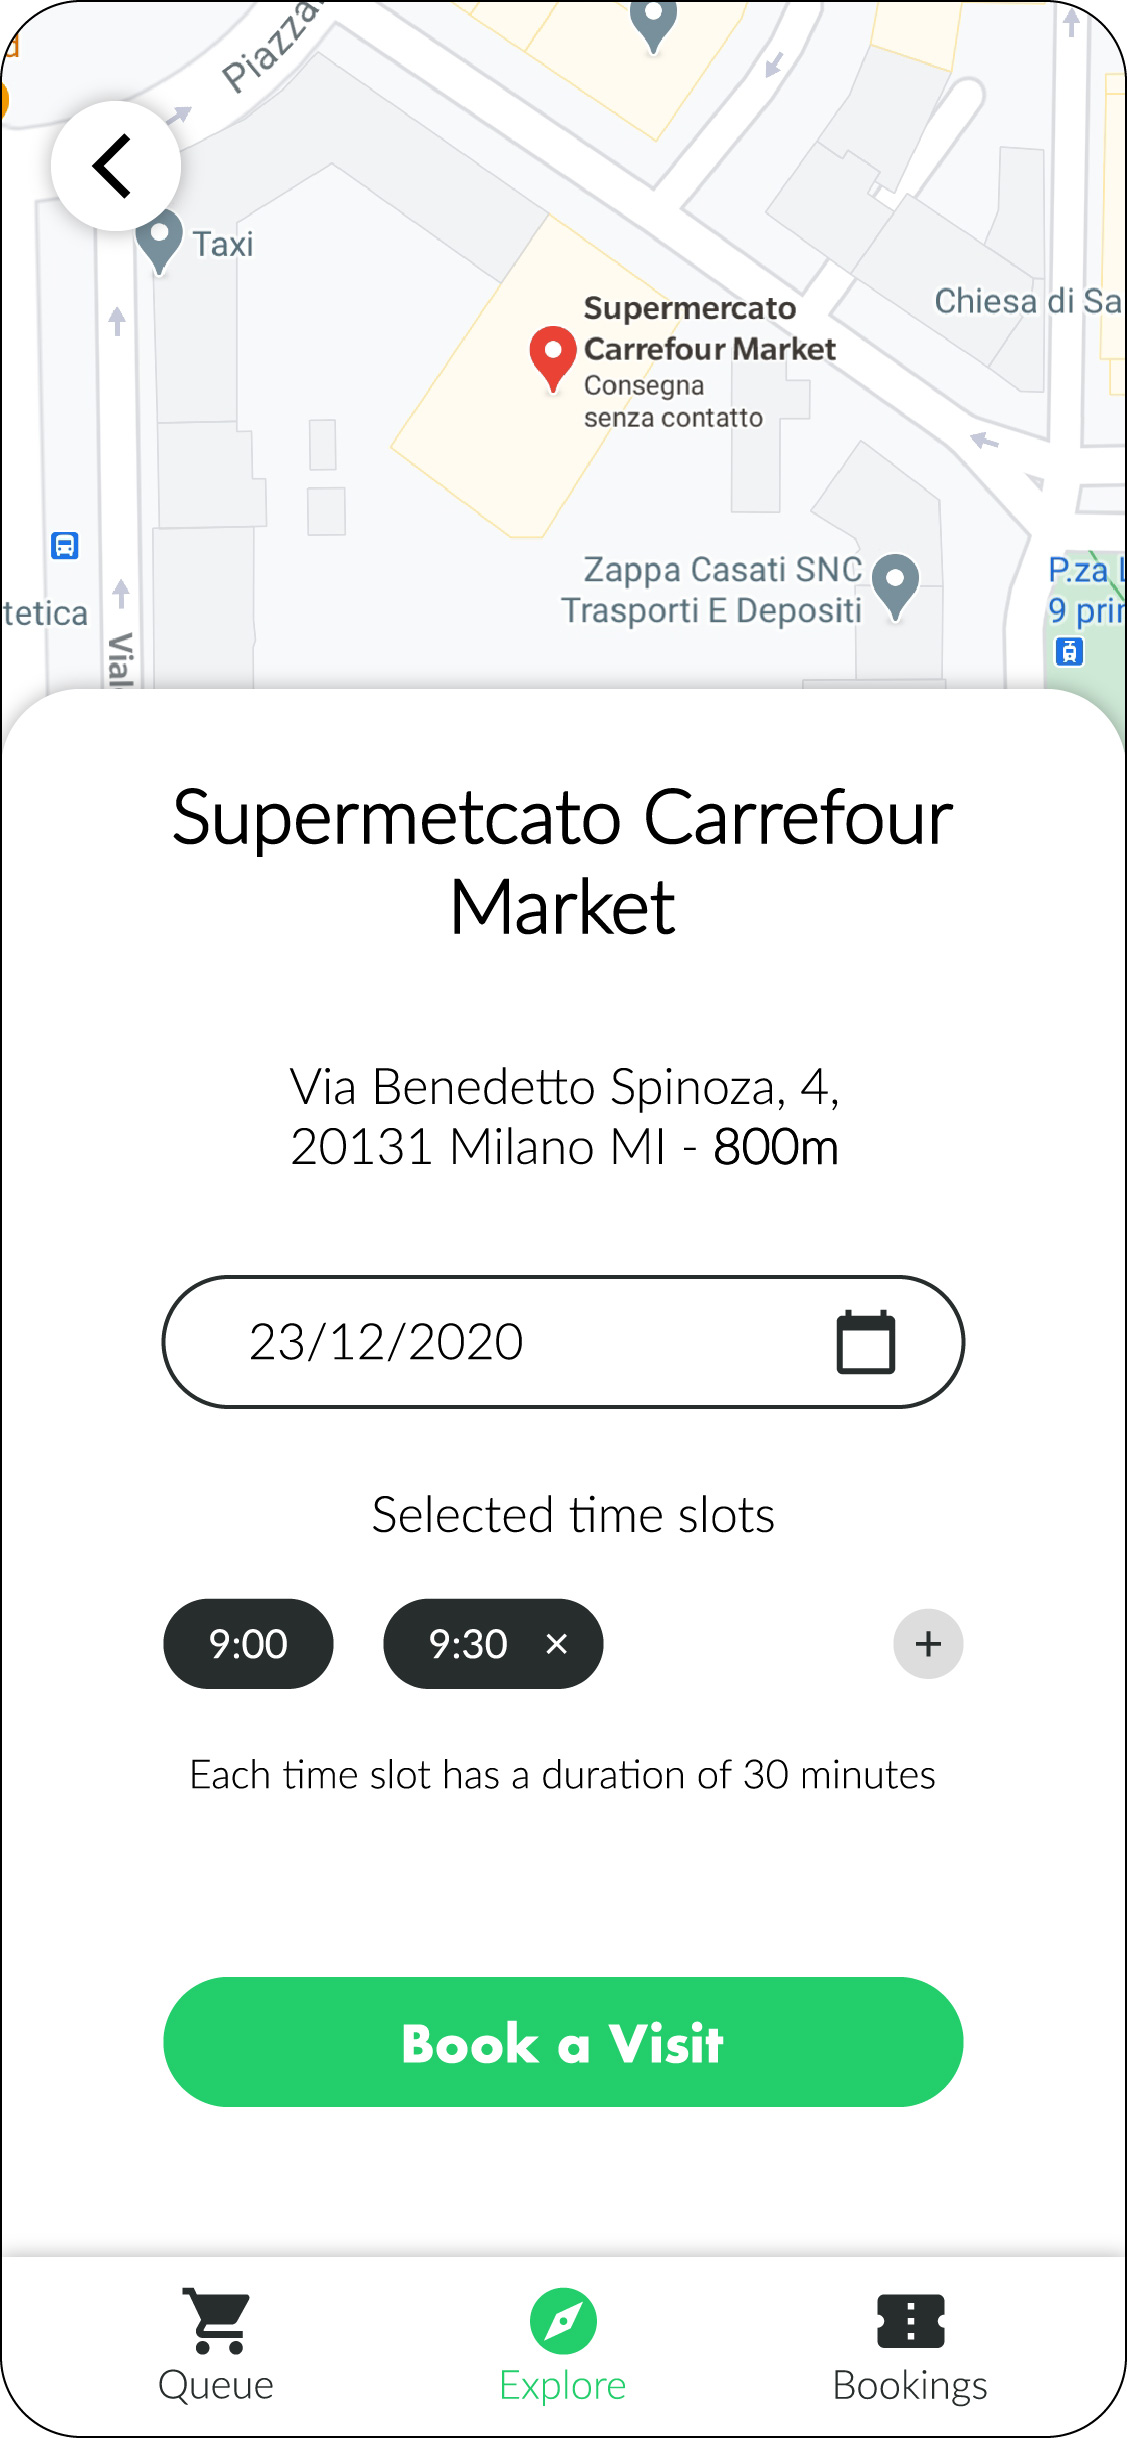
\includegraphics{../mockups/book}
        \caption*{New reservation page}
    \end{subfigure}
    \quad
    \begin{subfigure}[t]{0.28\textwidth} 
        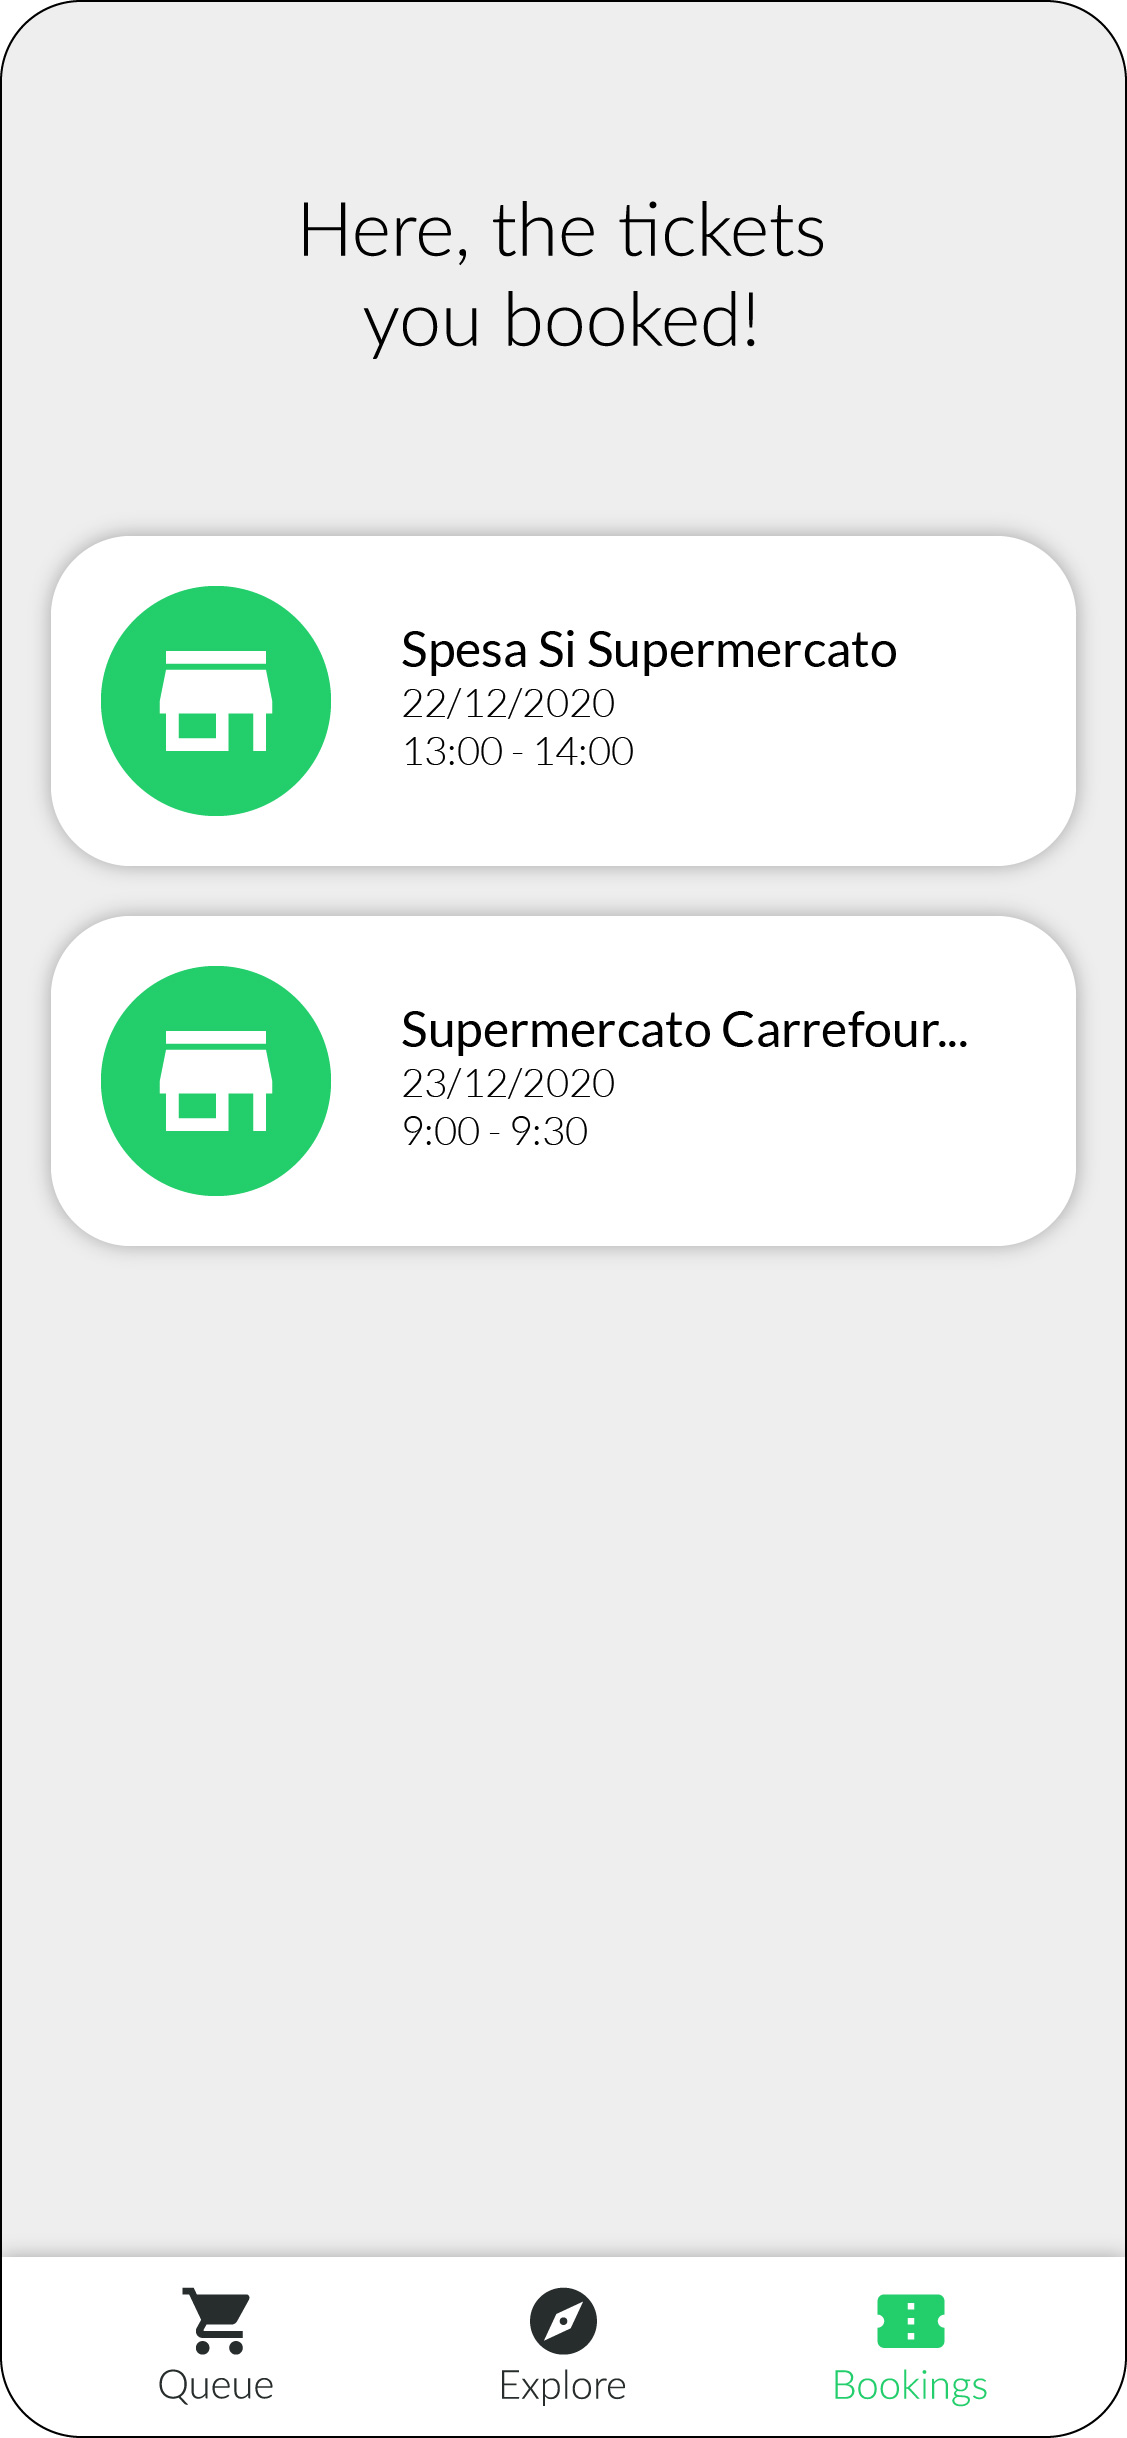
\includegraphics{../mockups/bookings}
        \caption*{Bookings page}
    \end{subfigure}
    \quad
    \begin{subfigure}[t]{0.28\textwidth} 
        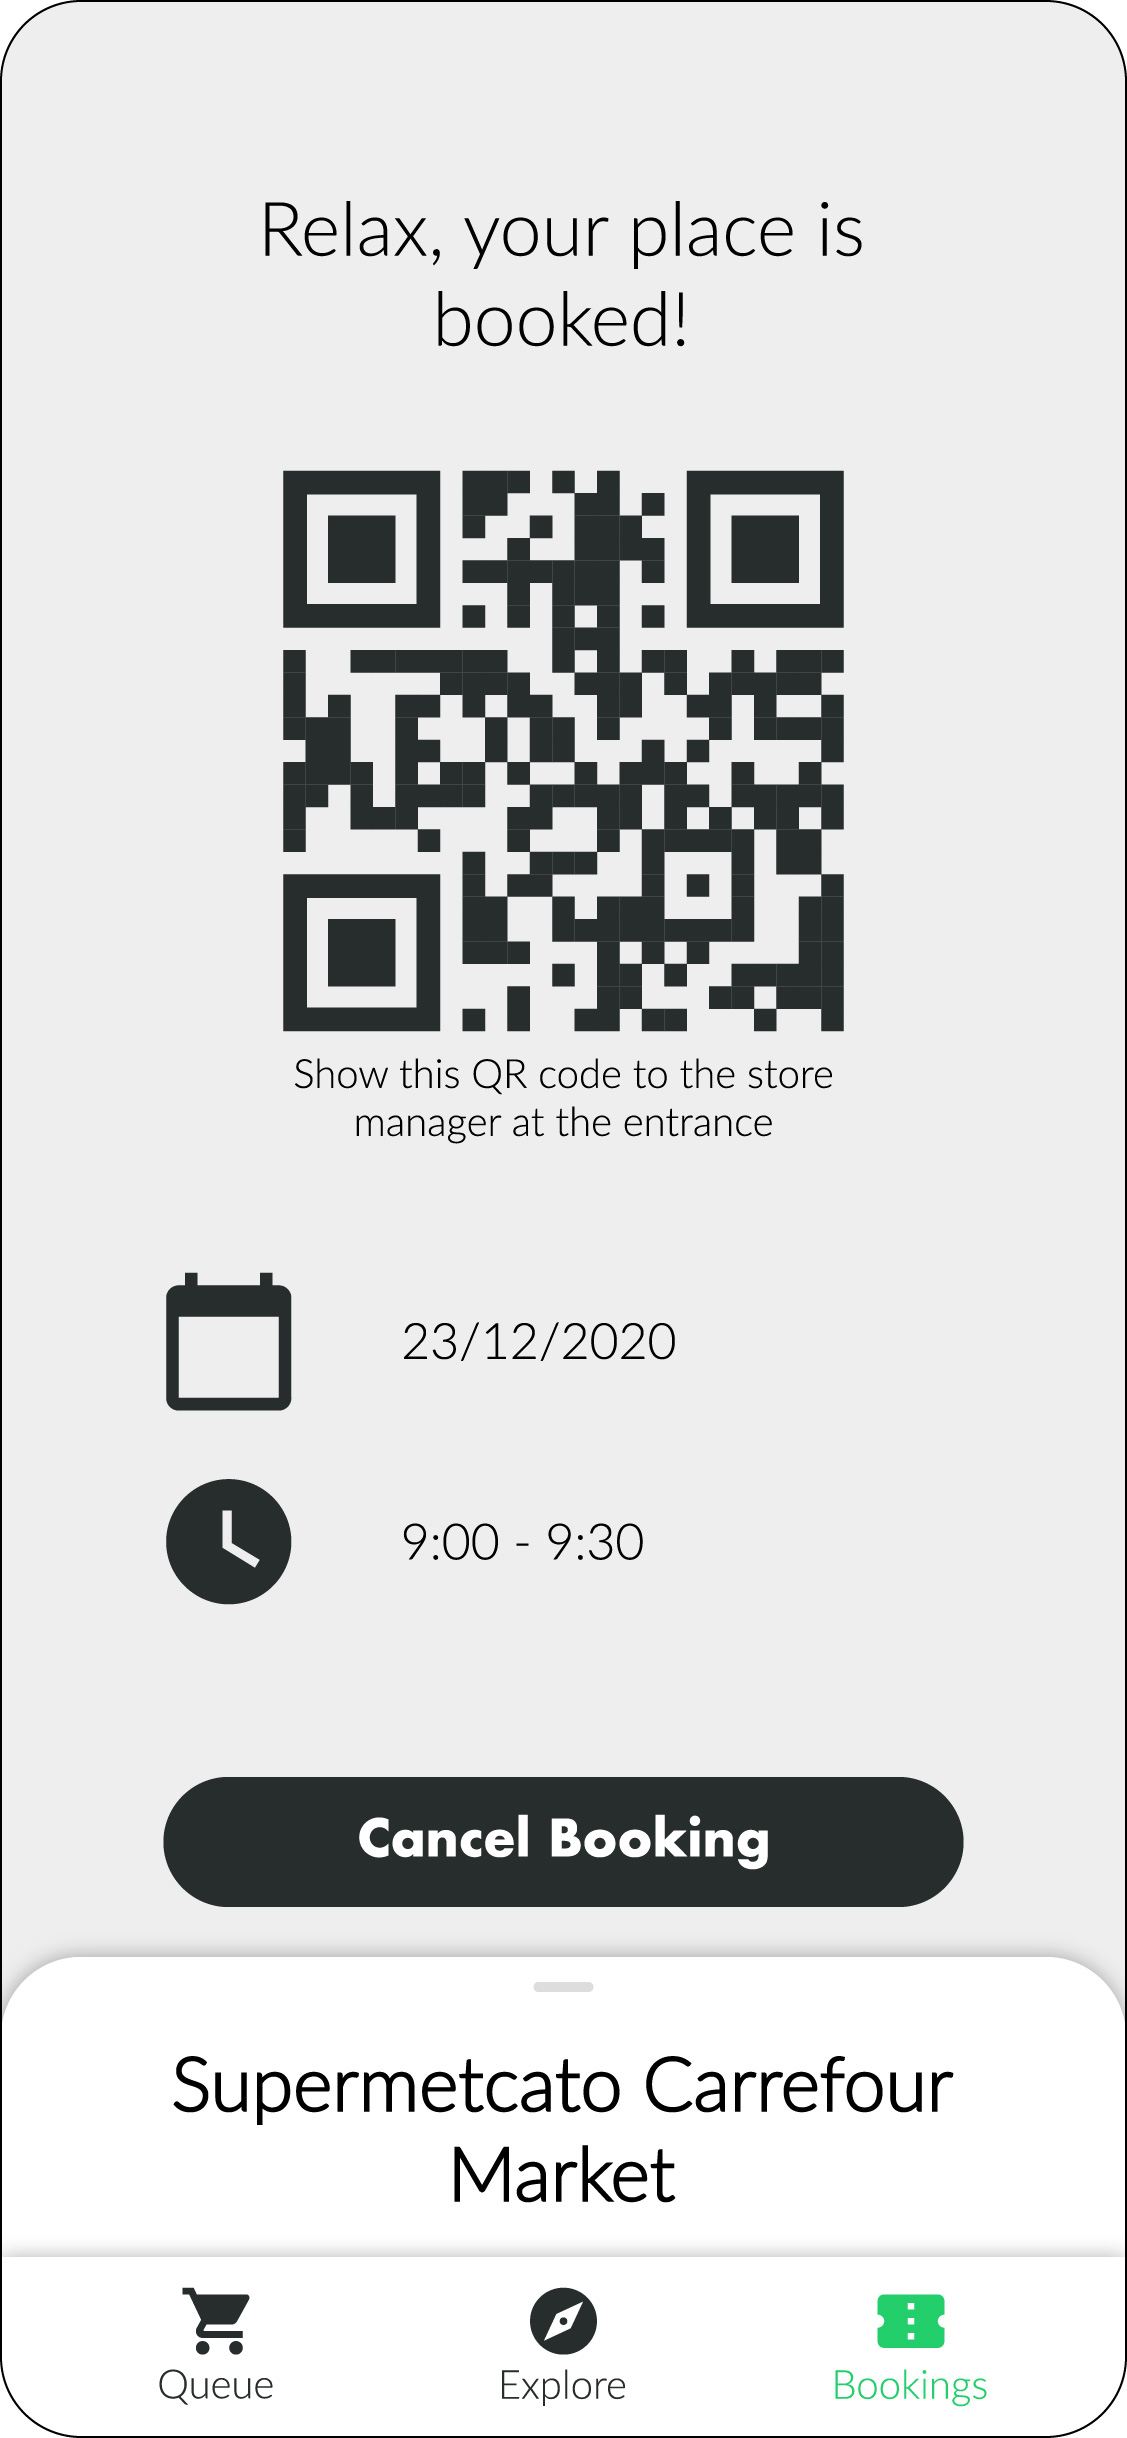
\includegraphics{../mockups/reservation}
        \caption*{Reservation page}
    \end{subfigure}
\end{figure}

\begin{figure}[H]
    \centering
    \begin{subfigure}[t]{0.28\textwidth} 
        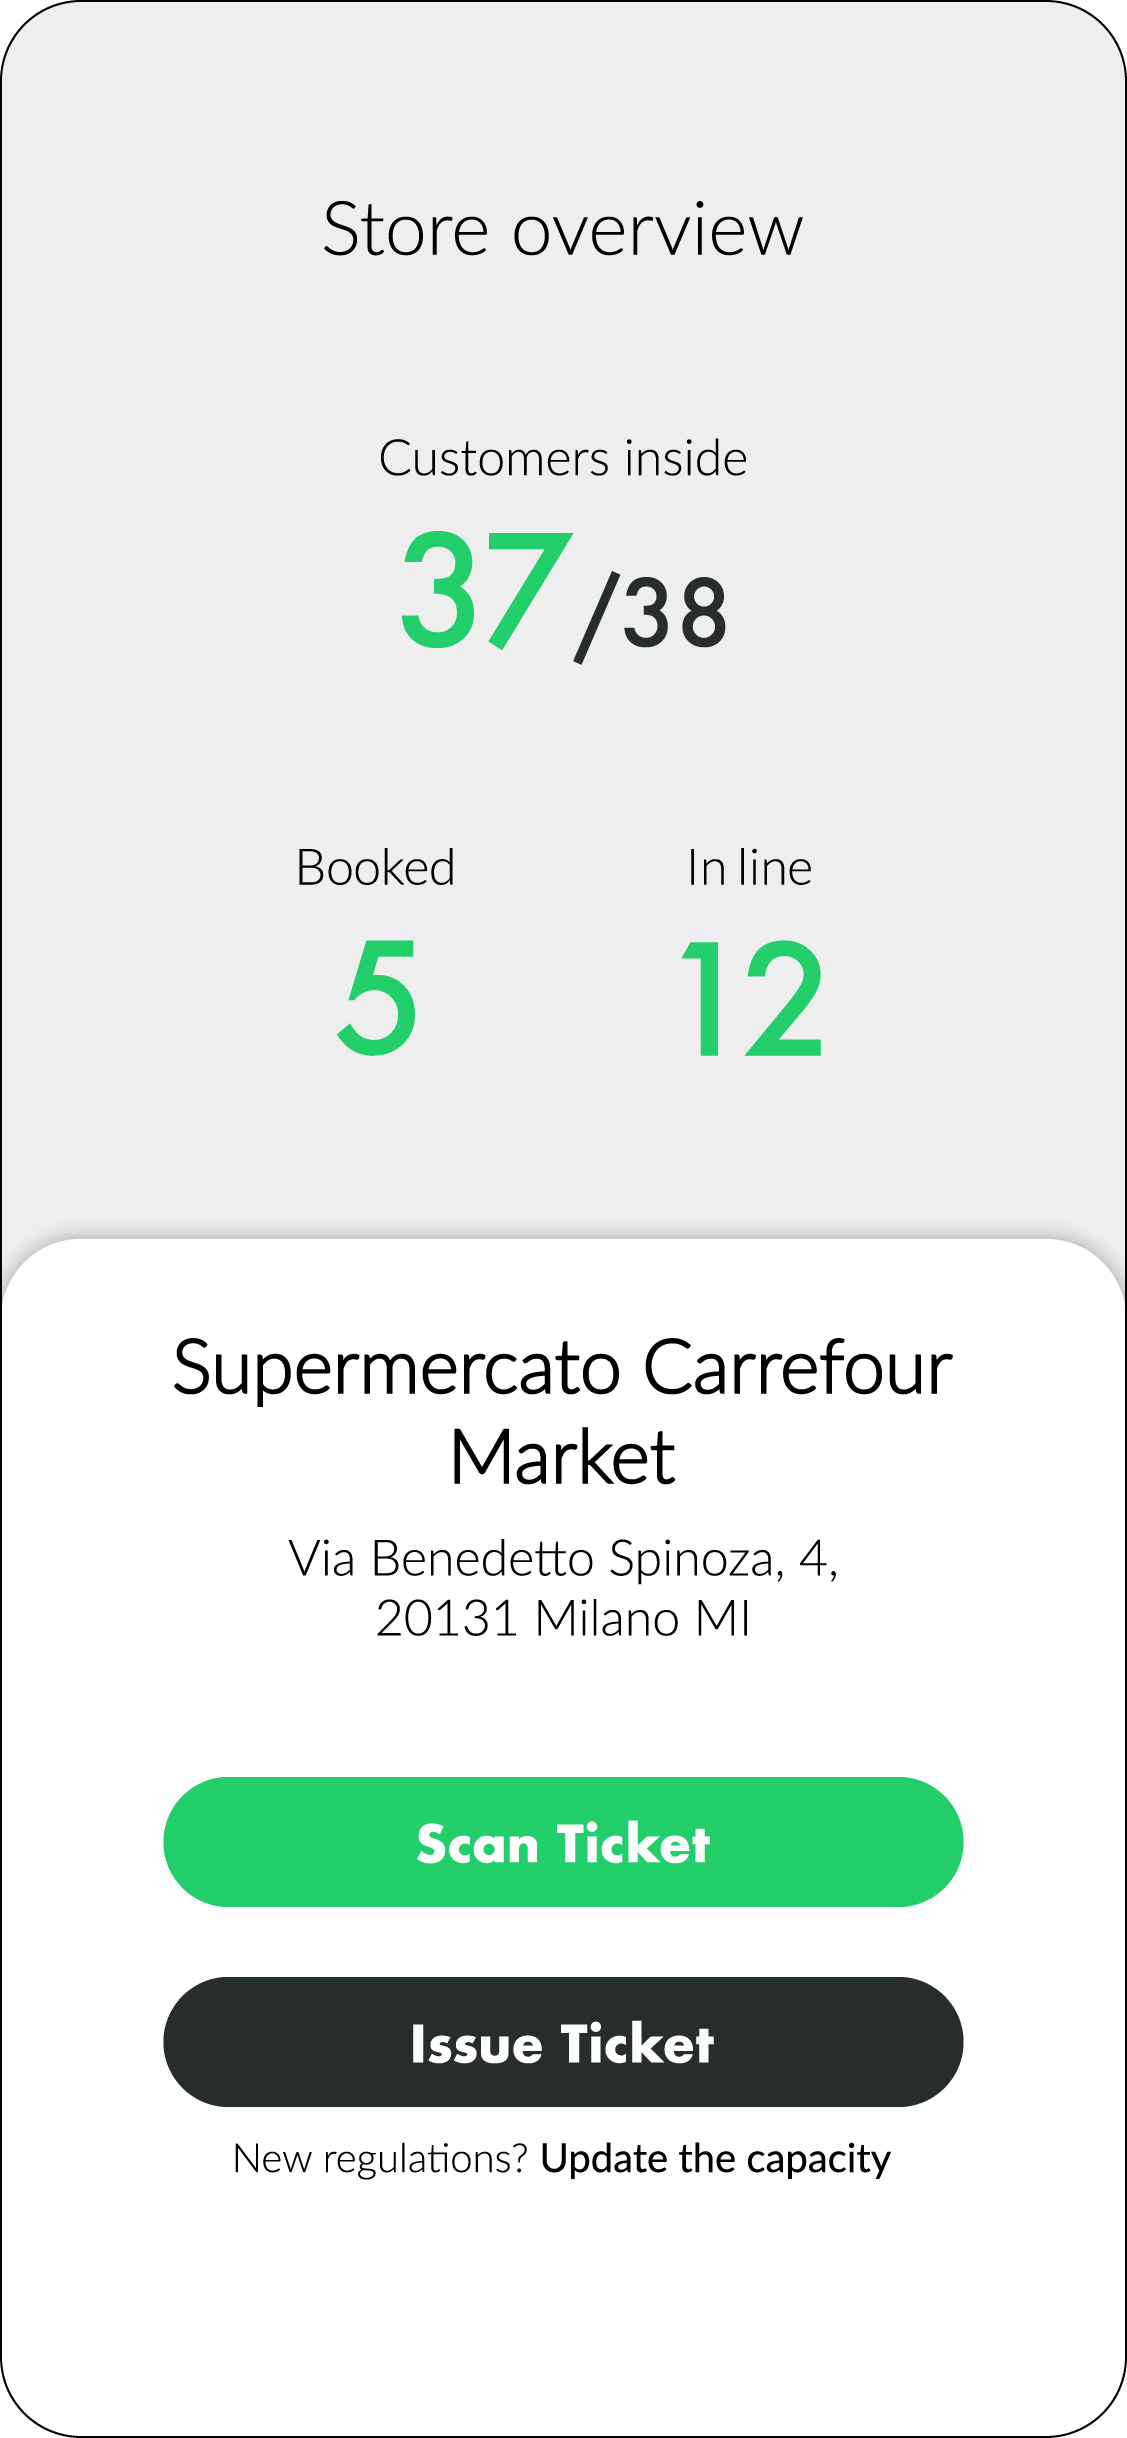
\includegraphics{../mockups/store_overview}
        \caption*{Store overview page}
    \end{subfigure}
    \quad
    \begin{subfigure}[t]{0.28\textwidth} 
        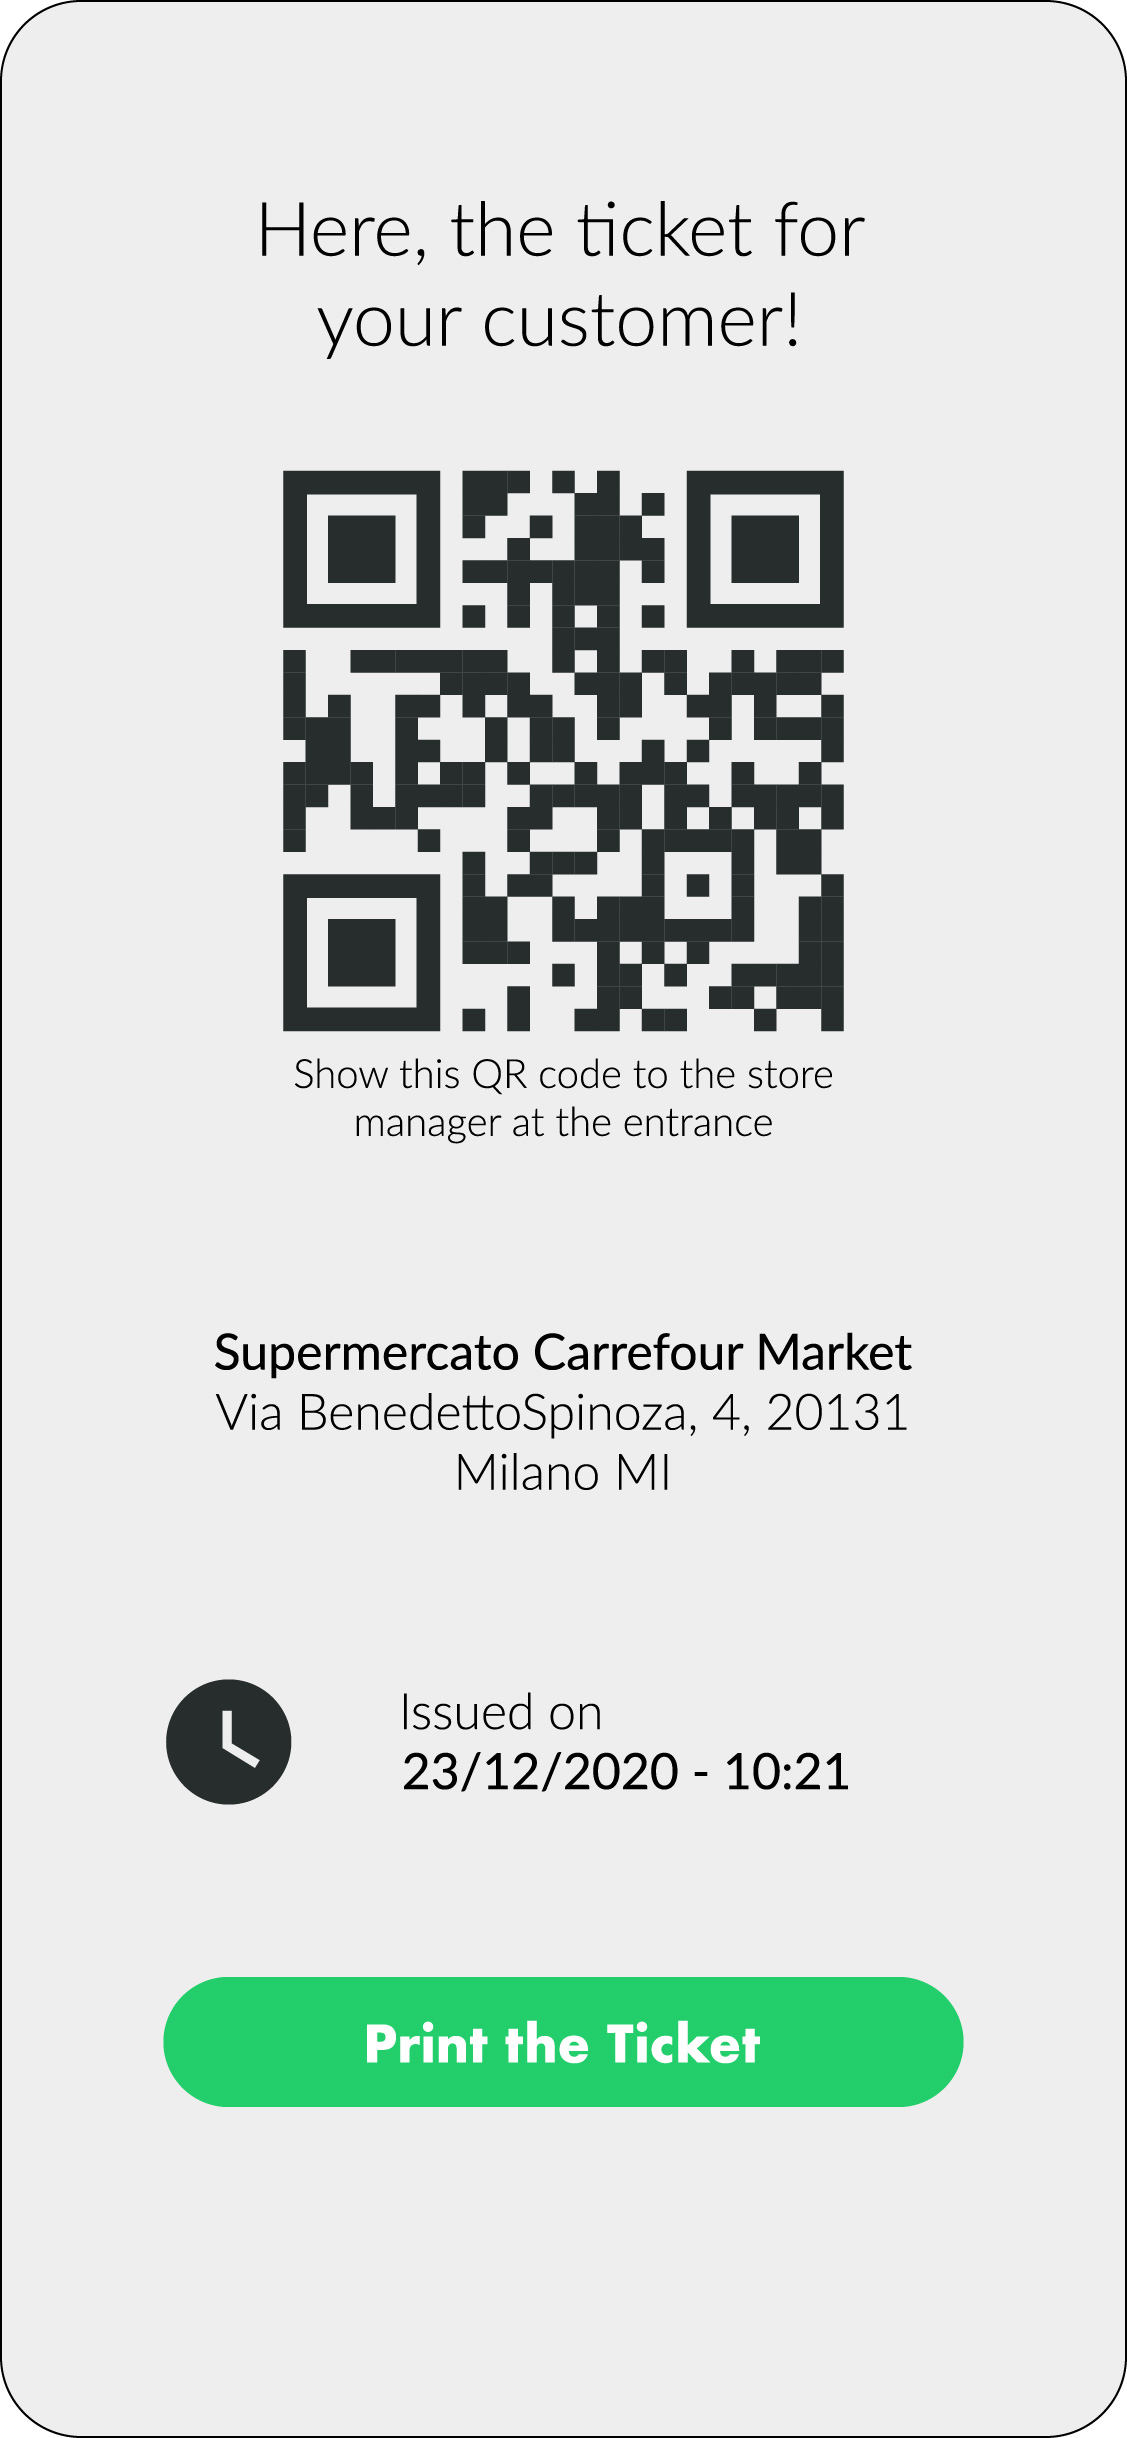
\includegraphics{../mockups/print_ticket}
        \caption*{Issued ticket page}
    \end{subfigure}
\end{figure}

\section{B. UX diagrams}

The following UX diagrams provide additional information about the journey of the various users inside the CLup web application.

The paths represented in the following diagrams take for granted the absence of exceptions of any kind. Each exception is handled as explained in the section \emph{3.B.1. Use cases} of the RASD.

Using the \emph{back} button provided by the web browser or the device will result in the default behaviour (previous page in history) and will therefore be ignored in this context.

\subsection{B.1. Visitor}

\begin{figure}[H]
\centering
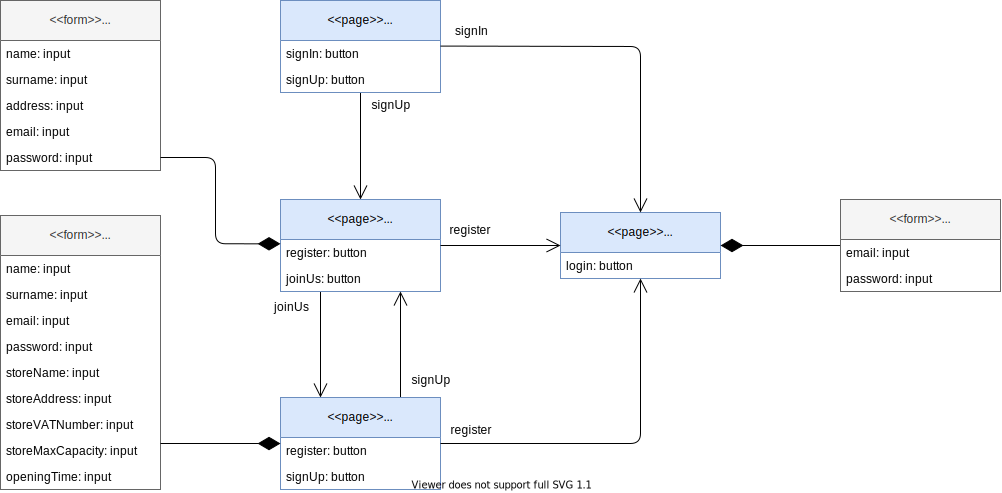
\includegraphics{ux_diagrams/ux_visitor}
\caption{Visitor diagram}
\end{figure}

The direct path from the \emph{Home} page to the \emph{UserLogin} page is considered as the default behaviour and therefore omitted in the next diagrams. The \emph{LoginCredentials} form is also not reported for clarity.

\subsection{B.2. Clupper}

\begin{figure}[H]
\centering
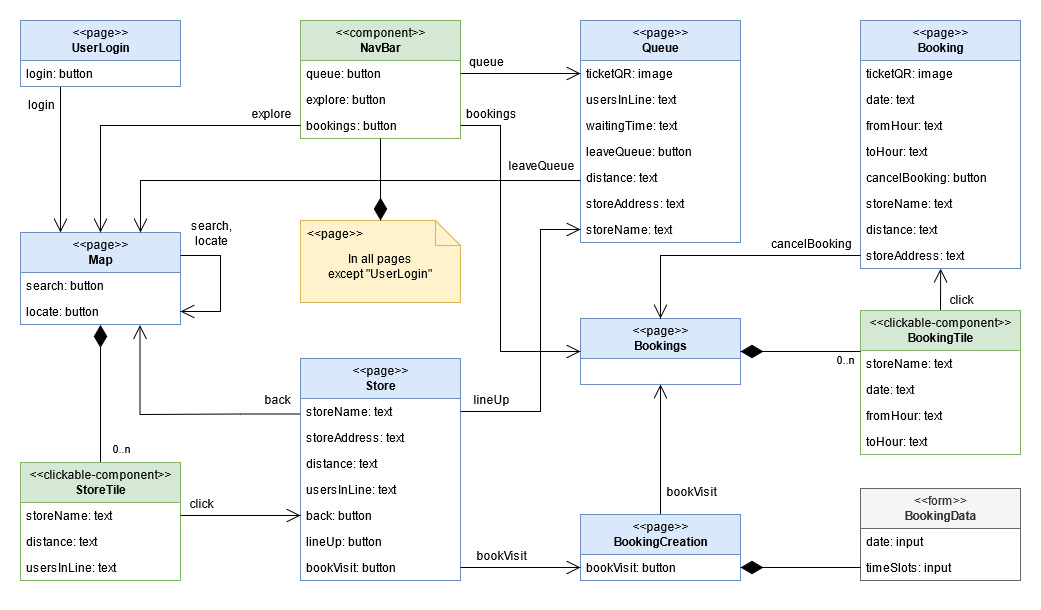
\includegraphics{ux_diagrams/ux_clupper}
\caption{Clupper diagram}
\end{figure}

The \emph{NavBar} component is included in every page accessible by the clupper except the ``UserLogin'' page, the arrow is omitted to improve readability.\\
The \emph{StoreTile} and \emph{BookingTile} can be included multiple times on the same page (with different data), they are classified as
\emph{clickable} since they behave like a button.

\subsection{B.3. Store manager}

\begin{figure}[H]
\centering
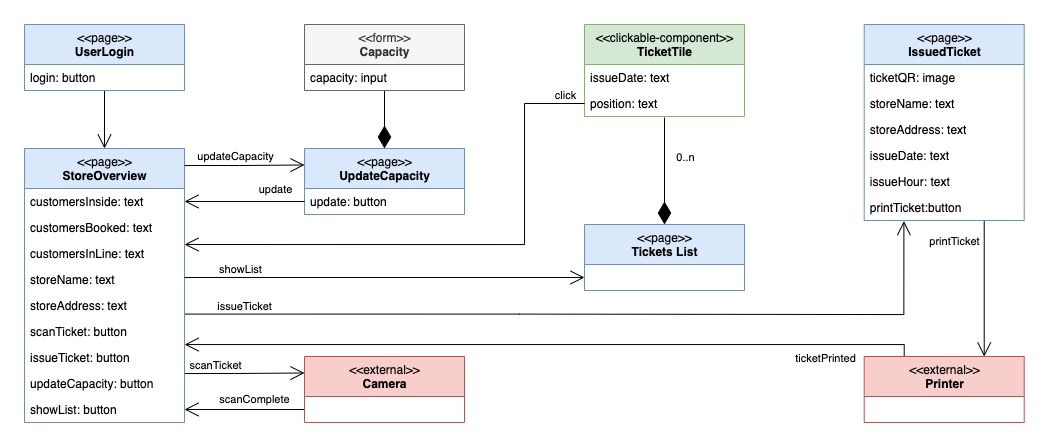
\includegraphics{ux_diagrams/ux_store_manager}
\caption{Store manager diagram}
\end{figure}

\emph{Camera} and \emph{Printer} represent the use of that specific external component (required for the correct functioning of the application) and have been included in the diagram to better clarify the sequence of actions that the store manager will perform.

\chapter{4. Requirements traceability}

While making the design choices presented in this document, the main objective was to fulfill in a complete and correct way the previously identified goals of the system.

Here is provided a mapping between the goals defined in the RASD and the system components illustrated in the DD.

\begin{itemize}
\item \textbf{G1}: Allow a clupper to join a store queue without having to physically approach the store.
    \begin{itemize}
        \item Account Services (\emph{Account Module})
        \item Clupper Services (\emph{Queue Module})
    \end{itemize}
\item \textbf{G2}: Allow a guest to join a store queue by requesting it to the store manager.
    \begin{itemize}
        \item Account Services (\emph{Account Module})
        \item Store Manager Services (\emph{Guest Module})
    \end{itemize}
\item \textbf{G3}: Allow a clupper to leave a store queue before entering.
    \begin{itemize}
        \item Account Services (\emph{Account Module})
        \item Clupper Services (\emph{Queue Module})
    \end{itemize}
\item \textbf{G4}: Allow a clupper to book a visit to the store.
    \begin{itemize}
        \item Account Services (\emph{Account Module})
        \item Clupper Services (\emph{Booking Module})
    \end{itemize}
\item \textbf{G5}: Allow a clupper to cancel a reservation to a store before entering.
    \begin{itemize}
        \item Account Services (\emph{Account Module})
        \item Clupper Services (\emph{Booking Module})
    \end{itemize}
\item \textbf{G6}: Allow a clupper to approach at the right time the store he has a ticket for.
    \begin{itemize}
        \item Account Services (\emph{Account Module})
        \item Clupper Services (\emph{Queue Module}, \emph{Booking Module})
    \end{itemize}
\item \textbf{G7}: Allow a store manager to have an overview of the store.
    \begin{itemize}
        \item Account Services (\emph{Account Module})
        \item Store Manager Services (\emph{Store Module})
    \end{itemize}
\item \textbf{G8}: Allow a store manager to regulate the entrances to the store.
    \begin{itemize}
        \item Account Services (\emph{Account Module})
        \item Store Manager Services (\emph{Store Module}, \emph{Ticket Module})
    \end{itemize}
\item \textbf{G9}: Allow a store manager to regulate the exits from the store.
    \begin{itemize}
        \item Account Services (\emph{Account Module})
        \item Store Manager Services (\emph{Store Module}, \emph{Ticket Module})
    \end{itemize}
\end{itemize}

\chapter{5. Implementation, integration and test plan}

TODO \emph{[Order in which we plan to implement the subcomponents and the order in which we plan to integrate them and test their integration]}

\chapter{6. Effort spent}

\section{Pair programming}

\begin{longtable}[]{@{}
  >{\raggedright\arraybackslash}p{(\columnwidth - 2\tabcolsep) * \real{0.8}}
  >{\raggedleft\arraybackslash}p{(\columnwidth - 2\tabcolsep) * \real{0.2}}@{}}
\toprule
Topic & Hours \\ \addlinespace
\midrule
\endhead
Architectural design diagrams & 3.5h \\ \addlinespace
\bottomrule
\end{longtable}

\section{Ferrara Alessandro}

\begin{longtable}[]{@{}
  >{\raggedright\arraybackslash}p{(\columnwidth - 2\tabcolsep) * \real{0.8}}
  >{\raggedleft\arraybackslash}p{(\columnwidth - 2\tabcolsep) * \real{0.2}}@{}}
\toprule
Topic & Hours \\ \addlinespace
\midrule
\endhead
Component Interface Diagrams & 1.0h \\ \addlinespace
Sequence Diagrams & 1.0h \\ \addlinespace
Section 2 & 2.0h \\ \addlinespace
\bottomrule
\end{longtable}

\section{Fratus Lorenzo}

\begin{longtable}[]{@{}
  >{\raggedright\arraybackslash}p{(\columnwidth - 2\tabcolsep) * \real{0.8}}
  >{\raggedleft\arraybackslash}p{(\columnwidth - 2\tabcolsep) * \real{0.2}}@{}}
\toprule
Topic & Hours \\ \addlinespace
\midrule
\endhead
UX diagrams & 2.0h \\ \addlinespace
DD structure & 1.0h \\ \addlinespace
Sections 2 and 3 & 2.5h \\ \addlinespace
Section 1 & 2.0h \\ \addlinespace
Section 4 & 1.0h \\ \addlinespace
\bottomrule
\end{longtable}

\chapter{7. References}

\begin{itemize}
\item
  Software Engineering II course slides
\item
  \href{https://www.gazzettaufficiale.it/atto/vediPermalink?atto.dataPubblicazioneGazzetta=2020-11-09\&atto.codiceRedazionale=20G00170\&tipoSerie=serie_generale\&tipoVigenza=originario\&tipoProvvedimento=*}{Decreto Ministeriale}
\end{itemize}

\end{document}